\documentclass[11pt]{article}
\usepackage[a4paper,margin=25mm,marginparwidth=20mm,marginparsep=10pt]{geometry}
\usepackage{fontspec}
\usepackage{amsmath,amssymb,mathtools}
\usepackage{unicode-math}
\usepackage[normalem]{ulem}
\usepackage{graphicx,xcolor,tikz,tikz-cd,pdflscape,needspace}
\usetikzlibrary{calc,decorations.pathmorphing,decorations.pathreplacing,arrows.meta,shapes.geometric}
\usepackage{newunicodechar,luacode,xurl}
\usepackage[hidelinks,unicode,hypertexnames=false]{hyperref}
\setmainfont{Latin Modern Roman}
\setmathfont{Latin Modern Math}
\setmathfont{STIX Two Math}[range={"27CB,"27CD}]
% Source boldsymbol calls all request Gamma; restore its actual bold glyph.
\renewcommand\boldsymbol[1]{\symbf{#1}}
\newfontfamily\cyrfont{STIX Two Text}[Scale=MatchLowercase]
\newunicodechar{А}{{\cyrfont\char"0410}}
\newunicodechar{Б}{{\cyrfont\char"0411}}
\newunicodechar{В}{{\cyrfont\char"0412}}
\newunicodechar{Г}{{\cyrfont\char"0413}}
\newunicodechar{Д}{{\cyrfont\char"0414}}
\newunicodechar{Е}{{\cyrfont\char"0415}}
\newunicodechar{Ж}{{\cyrfont\char"0416}}
\newunicodechar{З}{{\cyrfont\char"0417}}
\newunicodechar{И}{{\cyrfont\char"0418}}
\newunicodechar{Й}{{\cyrfont\char"0419}}
\newunicodechar{К}{{\cyrfont\char"041A}}
\newunicodechar{Л}{{\cyrfont\char"041B}}
\newunicodechar{М}{{\cyrfont\char"041C}}
\newunicodechar{Н}{{\cyrfont\char"041D}}
\newunicodechar{О}{{\cyrfont\char"041E}}
\newunicodechar{П}{{\cyrfont\char"041F}}
\newunicodechar{Р}{{\cyrfont\char"0420}}
\newunicodechar{С}{{\cyrfont\char"0421}}
\newunicodechar{Т}{{\cyrfont\char"0422}}
\newunicodechar{У}{{\cyrfont\char"0423}}
\newunicodechar{Ф}{{\cyrfont\char"0424}}
\newunicodechar{Х}{{\cyrfont\char"0425}}
\newunicodechar{Ц}{{\cyrfont\char"0426}}
\newunicodechar{Ч}{{\cyrfont\char"0427}}
\newunicodechar{Ш}{{\cyrfont\char"0428}}
\newunicodechar{Щ}{{\cyrfont\char"0429}}
\newunicodechar{Ъ}{{\cyrfont\char"042A}}
\newunicodechar{Ы}{{\cyrfont\char"042B}}
\newunicodechar{Ь}{{\cyrfont\char"042C}}
\newunicodechar{Э}{{\cyrfont\char"042D}}
\newunicodechar{Ю}{{\cyrfont\char"042E}}
\newunicodechar{Я}{{\cyrfont\char"042F}}
\newunicodechar{а}{{\cyrfont\char"0430}}
\newunicodechar{б}{{\cyrfont\char"0431}}
\newunicodechar{в}{{\cyrfont\char"0432}}
\newunicodechar{г}{{\cyrfont\char"0433}}
\newunicodechar{д}{{\cyrfont\char"0434}}
\newunicodechar{е}{{\cyrfont\char"0435}}
\newunicodechar{ж}{{\cyrfont\char"0436}}
\newunicodechar{з}{{\cyrfont\char"0437}}
\newunicodechar{и}{{\cyrfont\char"0438}}
\newunicodechar{й}{{\cyrfont\char"0439}}
\newunicodechar{к}{{\cyrfont\char"043A}}
\newunicodechar{л}{{\cyrfont\char"043B}}
\newunicodechar{м}{{\cyrfont\char"043C}}
\newunicodechar{н}{{\cyrfont\char"043D}}
\newunicodechar{о}{{\cyrfont\char"043E}}
\newunicodechar{п}{{\cyrfont\char"043F}}
\newunicodechar{р}{{\cyrfont\char"0440}}
\newunicodechar{с}{{\cyrfont\char"0441}}
\newunicodechar{т}{{\cyrfont\char"0442}}
\newunicodechar{у}{{\cyrfont\char"0443}}
\newunicodechar{ф}{{\cyrfont\char"0444}}
\newunicodechar{х}{{\cyrfont\char"0445}}
\newunicodechar{ц}{{\cyrfont\char"0446}}
\newunicodechar{ч}{{\cyrfont\char"0447}}
\newunicodechar{ш}{{\cyrfont\char"0448}}
\newunicodechar{щ}{{\cyrfont\char"0449}}
\newunicodechar{ъ}{{\cyrfont\char"044A}}
\newunicodechar{ы}{{\cyrfont\char"044B}}
\newunicodechar{ь}{{\cyrfont\char"044C}}
\newunicodechar{э}{{\cyrfont\char"044D}}
\newunicodechar{ю}{{\cyrfont\char"044E}}
\newunicodechar{я}{{\cyrfont\char"044F}}
\newunicodechar{≃}{\ensuremath{\simeq}}
\newattribute\LMattr
\newcount\LMform
\newcount\LMinApp
\LMform=2
\LMinApp=0
\newcommand\LMlanguage{en}
\newcommand\LMcotename{}
\newcommand\LMcote[1]{\gdef\LMcotename{#1}}
\newcommand\LMnotelabel{Marginal note}
\newcommand\LMappheading{Apparatus for this scan}
\newcommand\LMdoubtheading{Uncertainty retained from cancelled passages}
\newcommand\LMmanuscriptlabel{Manuscript}
\newcommand\LMcorrectedlabel{Text}
\newcommand\LMreasonlabel{Reason}
\newcommand\LMomittedlabel{omitted}
\newcommand\LMinsertedlabel{insertion integrated}
\newcommand\LMlayoutlabel{Diagram continued on the landscape page}
\newcommand\LMvarref[1]{\ifmmode\else\ifinner\else\textsuperscript{\textcolor{gray}{\LMreftext{#1}}}\fi\fi}
\newcommand\LMreftext[1]{\directlua{LM.reftext("\luaescapestring{#1}")}}
\newcommand\var[4]{\ifcase\LMform #1\or #2\ifnum\LMinApp=0\LMvarref{#4}\fi\or #2\fi}
\newcommand\LMadded[1]{{\color{teal}#1}}
\newcommand\deleted[1]{{\color{gray}#1}}
\newcommand\inserted[1]{{\color{teal}#1}}
\newcommand\LMarchivefooter[3]{#2}
\newcommand\LMsourceid{}
\newcommand\LMsourceMark[2]{{\def\LMsourceid{#1}#2}}
\newcommand\LMmark[1]{\directlua{LM.mark("#1",tex.inputlineno)}}
\newcommand\unsure[1]{{\color{blue}\LMmark{unsure}#1}}
\newcommand\illegible[1]{{\LMmark{illegible}\textcolor{red}{[illeg.~#1]}}}
\newcommand\LMuncertaindeletion[1]{{\color{blue}\LMmark{cancelled-anchor}\ensuremath{\dagger}}}
\newcommand\LMdoubtcopy[1]{{\color{blue}\LMmark{residual-unsure}#1}}
\newcommand\LMdoubtdata[1]{}
\newcommand\LMcancelledDoubts[1]{\ifnum\LMform=2{\color{blue}\LMmark{cancelled-anchor}\ensuremath{\dagger}}\fi}
\newcommand\scanpage[1]{%
 \par\LMflushnotes\LMflushpages\smallskip\directlua{LM.at("\luaescapestring{\LMcotename}","\luaescapestring{\detokenize{#1}}")}%
 \ifnum\LMform=2\noindent\marginpar{\footnotesize\raggedright\LMmark{scan}\textcolor{gray}{[scan #1]}}%
 \else\noindent{\footnotesize\LMmark{scan}\textcolor{gray}{[scan #1]}}\par\nobreak\fi}
\newcommand\mspage[1]{\ifnum\LMform=2\ifinner\LMqueuepage{#1}\else\marginpar{\footnotesize\raggedright\textcolor{gray}{[p.~#1]}}\fi\else{\footnotesize\textcolor{gray}{[p.~#1]}}\ \fi}
\newcommand\diagram[1]{\ifmmode\vcenter{\hbox{#1}}\else\ifinner #1\else\par\begin{center}#1\end{center}\par\LMflushnotes\LMflushpages\fi\fi}
\let\figure\relax\newcommand\figure[1]{\ifmmode\vcenter{\hbox{#1}}\else\ifinner #1\else\par\begin{center}#1\end{center}\par\LMflushnotes\LMflushpages\fi\fi}
\newcommand\LMpagefigure[2]{\ifnum\LMform=2\marginpar{\footnotesize\raggedright\textcolor{gray}{\textcircled{#2}}}\else#1\fi}
\newcommand\LMmathnotice[1]{\par\noindent{\footnotesize\color{gray}[\ensuremath{\hookrightarrow}\ #1]}\par}
\newcommand\LMlayoutnotice[1]{\par\noindent{\footnotesize\color{gray}[\LMlayoutlabel; #1]}\par}
\tolerance=1200
\emergencystretch=3em
\tracinglostchars=3
\hfuzz=0pt
\vfuzz=0pt
\raggedbottom
\setcounter{tocdepth}{1}
\setlength\parindent{1.3em}
\setlength\parskip{1.5pt plus 1pt}
\allowdisplaybreaks[2]
\begin{luacode*}
-- Marked passages are linked at shipout, including paragraphs and mathematics.
-- No node, line, display or font is scaled by this code.
LM = {measure=false, maxw=0, markers={}, links=0, pages=0, scanmap={}, trial_overfull=0, shortnotes=0, blocknotes=0}
local F=LM
local A=luatexbase.registernumber('LMattr')
local HLIST,VLIST,GLUE,KERN,WHATSIT,GLYPH,PENALTY,MATH = node.id('hlist'),node.id('vlist'),node.id('glue'),node.id('kern'),node.id('whatsit'),node.id('glyph'),node.id('penalty'),node.id('math')
local STARTLINK,ENDLINK,ACTION=node.subtype('pdf_start_link'),node.subtype('pdf_end_link'),node.subtype('pdf_action')
local inert={[GLUE]=true,[KERN]=true,[PENALTY]=true,[WHATSIT]=true,[MATH]=true}
function F.at(cote,scan)
 F.cote=cote;F.scan=tonumber(string.match(scan,'^%s*(%d+)')) or 0
end
F.by_source={}
function F.mark(kind,line)
 if F.measure or not F.cote or not F.scan or F.scan==0 then return end
 local parent=tex.attribute[A]
 if not parent or parent<1 then parent=0 end
 local source=token.get_macro('LMsourceid') or ''
 if source=='' then source='auto:'..kind..':'..F.cote..':'..F.scan..':'..line end
 local id=F.by_source[source]
 if not id then
  id=#F.markers+1;F.by_source[source]=id
  F.markers[id]={id=id,source=source,kind=kind,cote=F.cote,scan=F.scan,line=line,parent=parent,runs=0,pages={},expansions=0}
 end
 local mark=F.markers[id]
 if parent~=id then mark.parent=parent end
 mark.expansions=mark.expansions+1
 tex.attribute[A]=id
end
local function url(m)
 return 'https://grothendieck.umontpellier.fr/web/viewer.html?file=../'..m.cote..'.pdf#page='..m.scan
end
local function collect(n,ids)
 local v=node.has_attribute(n,A)
 if v and v>0 then ids[v]=true end
 if (n.id==HLIST or n.id==VLIST) and n.head then for q in node.traverse(n.head) do collect(q,ids) end end
end
local function cover(id)
 local m=F.markers[id]
 if not m then return end
 m.runs=m.runs+1;m.pages[F.pages]=true
 local key=m.cote..':'..m.scan
 F.scanmap[key]=F.scanmap[key] or {};F.scanmap[key][F.pages]=true
 if m.parent>0 then cover(m.parent) end
end
local link_lists
local function link_runs(box)
 local n=box.head
 while n do
  local v=node.has_attribute(n,A)
  if v and v>0 and F.markers[v] and not inert[n.id] then
   local last,m=n,n.next
   while m do
    if inert[m.id] then
    elseif node.has_attribute(m,A)==v then last=m
    else break end
    m=m.next
   end
   local ids={};local q=n
   while q do collect(q,ids);if q==last then break end;q=q.next end
   local sorted={};for id in pairs(ids) do sorted[#sorted+1]=id;cover(id) end;table.sort(sorted)
   local w,h,d=node.dimensions(box.glue_set,box.glue_sign,box.glue_order,n,last.next)
   local s=node.new(WHATSIT,STARTLINK);s.width=w;s.height=h;s.depth=d
   local a=node.new(WHATSIT,ACTION);a.action_type=3
   a.data='/Subtype/Link/Border[0 0 0]/NM(LM'..table.concat(sorted,',')..')/A<</Type/Action/S/URI/URI('..url(F.markers[v])..')>>'
   s.action=a
   local e=node.new(WHATSIT,ENDLINK)
   box.head=node.insert_before(box.head,n,s);node.insert_after(box.head,last,e)
   F.links=F.links+1;n=e.next
  else
   if n.id==HLIST then link_runs(n) elseif n.id==VLIST then link_lists(n) end
   n=n.next
  end
 end
end
link_lists=function(box)
 for n in node.traverse(box.head) do
  if n.id==HLIST then link_runs(n) elseif n.id==VLIST then link_lists(n) end
 end
end
luatexbase.add_to_callback('pre_shipout_filter',function(box)
 F.pages=F.pages+1
 if box.id==HLIST then link_runs(box) elseif box.id==VLIST then link_lists(box) end
 return true
end,'lm.scanlinks')
-- Only discarded margin trials are measured; actual pages are never fitted.
luatexbase.add_to_callback('post_linebreak_filter',function(head)
 if F.measure then
  for line in node.traverse_id(HLIST,head) do
   if line.head then
    local nw=node.dimensions(line.glue_set,line.glue_sign,line.glue_order,line.head)
    if nw>F.maxw then F.maxw=nw end
   end
  end
 end
 return head
end,'lm.measure.margin')
-- hpack_quality replaces the engine's reporter; every actual overfull is
-- reported, with its exact width and input lines. Discarded trials are separate.
luatexbase.add_to_callback('hpack_quality',function(incident,detail,head,first,last)
 if incident=='overfull' then
  if F.measure then F.trial_overfull=F.trial_overfull+1
  else texio.write_nl('term and log',string.format('Overfull \\hbox (%.5fpt too wide) at lines %d--%d',detail/65536,first,last)) end
 elseif incident=='underfull' and not F.measure and detail>=1000 then
  texio.write_nl('log',string.format('Underfull \\hbox (badness %d) at lines %d--%d',detail,first,last))
 end
end,'lm.quality.report')
function F.summary()
 local f=assert(io.open(tex.jobname..'.lm-links.tsv','w'))
 f:write('marker\tkind\tcote\tscan\ttex_line\tparent\tlinked_runs\tphysical_pages\tsource_id\texpansions\n')
 local missing=0
 for _,m in ipairs(F.markers) do
  local ps={};for p in pairs(m.pages) do ps[#ps+1]=p end;table.sort(ps)
  if m.runs==0 then missing=missing+1 end
  f:write(table.concat({m.id,m.kind,m.cote,m.scan,m.line,m.parent,m.runs,table.concat(ps,','),m.source,m.expansions},'\t'),'\n')
 end
 f:close()
 local g=assert(io.open(tex.jobname..'.lm-scans.tsv','w'));g:write('cote\tscan\tphysical_pages\tsource_id\texpansions\n')
 local ks={};for k in pairs(F.scanmap) do ks[#ks+1]=k end;table.sort(ks)
 for _,k in ipairs(ks) do
  local cote,scan=string.match(k,'(.*):(%d+)');local ps={};for p in pairs(F.scanmap[k]) do ps[#ps+1]=p end;table.sort(ps)
  g:write(cote,'\t',scan,'\t',table.concat(ps,','),'\n')
 end;g:close()
 texio.write_nl('term and log',string.format('LM-AUDIT markers=%d links=%d unlinked=%d scans=%d pages=%d margin_short=%d margin_block=%d discarded_trial_overfull=%d',#F.markers,F.links,missing,#ks,F.pages,F.shortnotes,F.blocknotes,F.trial_overfull))
end

function LM.reftext(s)
 local a,b=string.match(s,'([A-Z])0*(%d+)$')
 tex.sprint(a and (string.lower(a)..b) or '*')
end

LM.noteids={};LM.nextnote=0;LM.pageids={}
function LM.noteref(source)
 if source=='' then source='note:'..tex.inputlineno end
 local id=LM.noteids[source]
 local fresh=0
 if not id then LM.nextnote=LM.nextnote+1;id=LM.nextnote;LM.noteids[source]=id;fresh=1 end
 tex.sprint('\\def\\LMcurrentnoteref{'..id..'}\\LMnotefresh='..fresh..'\\relax')
end
function LM.pagequeue(source)
 local fresh=0
 if not LM.pageids[source] then LM.pageids[source]=true;fresh=1 end
 tex.count.LMnotefresh=fresh
end

\end{luacode*}
\makeatletter
\AtBeginDocument{\let\LMsimeq\simeq\protected\def\simeq{\ifmmode\LMsimeq\else$\LMsimeq$\fi}%
 \let\LMGamma\Gamma\protected\def\Gamma{\ifmmode\LMGamma\else$\LMGamma$\fi}}
\output\expandafter{\expandafter\unsetattribute\expandafter\LMattr\the\output}
\AtEndDocument{\clearpage\directlua{LM.summary()}}
\newif\ifLMtrial
\newcount\LMnotefresh
\newcommand\LMcurrentnoteref{}
\newcommand\LMgetnoteref{\directlua{LM.noteref("\luaescapestring{\LMsourceid}")}}
\newsavebox\LMmbox
\newdimen\LMmw
\newdimen\LMmh
\newdimen\LMnotewidth
\newcommand\LMmarginstyle{\footnotesize\rightskip=0pt plus 2.5em\relax\parfillskip=0pt plus 1fil\relax\hyphenpenalty=50\relax\def\margin##1{{[##1]}}}
\newcommand\LMtrial[2]{%
 \LMtrialtrue\directlua{LM.measure=true LM.maxw=0}%
 \setbox\LMmbox\vbox{\hsize=#1\relax\@parboxrestore\LMmarginstyle #2\par}%
 \LMtrialfalse\directlua{LM.measure=false tex.setdimen("LMmw",LM.maxw)}%
 \LMmh=\dimexpr\ht\LMmbox+\dp\LMmbox\relax}
\newcommand\LMinblock[1]{%
 \directlua{LM.blocknotes=LM.blocknotes+1}%
 \par\smallskip\noindent{\color{gray}\rule{.20\linewidth}{.35pt}}\par\nobreak
 \begingroup\LMmarginstyle\parindent=0pt\noindent\textit{\LMnotelabel.}\enspace #1\par\endgroup\smallskip}
\newcommand\LMmargin[1]{\begingroup\LMgetnoteref
 \LMtrial{\marginparwidth}{#1}%
 \ifdim\LMmw>\marginparwidth\LMnotemark{\LMcurrentnoteref}\LMinblock{\textsuperscript{m\LMcurrentnoteref}\ #1}%
 \else\ifdim\LMmh>33pt\LMnotemark{\LMcurrentnoteref}\LMinblock{\textsuperscript{m\LMcurrentnoteref}\ #1}%
 \else\directlua{LM.shortnotes=LM.shortnotes+1}\marginpar{\LMmarginstyle #1}%
 \fi\fi\endgroup}
% This source-local wrapper retains both consecutive short notes on separate lines.
\newcommand\LMpairedmargins[1]{\begingroup
 \marginpar{\LMmarginstyle
  \def\margin##1{\LMgetnoteref\directlua{LM.shortnotes=LM.shortnotes+1}\noindent##1\par}#1}%
 \endgroup}
\newcounter{LMnoteref}
\newcommand\LMpendingnotes{}
\newcommand\LMpendingpages{}
\newcommand\LMqueuepage[1]{\ifLMtrial\else\directlua{LM.pagequeue("\luaescapestring{\LMsourceid}")}\ifnum\LMnotefresh=1\g@addto@macro\LMpendingpages{\marginpar{\footnotesize\raggedright\textcolor{gray}{[p.~#1]}}}\fi\fi}
\newcommand\LMflushpages{\ifinner\else\LMpendingpages\global\let\LMpendingpages\@empty\fi}
\newcommand\LMnotemark[1]{\ifmmode{}^{\scriptscriptstyle\text{\color{gray}m#1}}\else\textsuperscript{\color{gray}m#1}\fi}
\newcommand\LMqueuenote[1]{%
 \LMgetnoteref\LMnotemark{\LMcurrentnoteref}%
 \ifnum\LMnotefresh=1\begingroup\edef\LMnext{\endgroup\noexpand\g@addto@macro\noexpand\LMpendingnotes{\noexpand\LMqueuednote{\LMcurrentnoteref}{\the\LMattr}{\unexpanded{#1}}}}\LMnext\fi}
\newcommand\LMqueuednote[3]{\begingroup\LMattr=#2\relax\ifnum#2>0\color{blue}\fi\LMinblock{\textsuperscript{m#1}\ #3}\endgroup}
\newcommand\LMflushnotes{\ifinner\else\begingroup\let\LMnextnotes\LMpendingnotes\global\let\LMpendingnotes\@empty\LMnextnotes\endgroup\fi}
\newcommand\margin[1]{\ifmmode\LMqueuenote{\(#1\)}\else\ifinner\LMqueuenote{#1}\else\LMmargin{#1}\fi\fi}
\AddToHook{env/equation*/after}{\LMflushnotes\LMflushpages}
\AddToHook{env/equation/after}{\LMflushnotes\LMflushpages}
\AddToHook{env/align*/after}{\LMflushnotes\LMflushpages}
\AddToHook{env/align/after}{\LMflushnotes\LMflushpages}
\AddToHook{env/gather*/after}{\LMflushnotes\LMflushpages}
\AddToHook{env/center/after}{\LMflushnotes\LMflushpages}
\makeatother
\newenvironment{LMapparatus}{\par\smallskip\begingroup\LMinApp=1\footnotesize\noindent\textcolor{gray}{\rule{.26\linewidth}{.35pt}}\par\noindent\textbf{\LMappheading}\par\smallskip}{\par\endgroup}
\newcommand\LMentry[6]{\par\noindent{\color{gray}\texttt{#1}}\enspace\textit{#2.}\enspace\textit{\LMmanuscriptlabel:}\enspace #3\par\noindent\textit{\LMcorrectedlabel:}\enspace #4\enspace\textit{\LMreasonlabel:}\enspace #5\par\smallskip}
\newcommand\LMcarryover[2]{\par\noindent{\scriptsize\color{gray}\texttt{#1}}\enspace #2\par}

\hypersetup{pdftitle={La Longue Marche à travers la théorie de Galois — Reading text},pdfauthor={Alexander Grothendieck}}
\begin{document}
% COMMON MASTER BODY SHA256 40c8ee32f3b10c855302ef74c32a81403699c368c04140780c644f1e76042c80
\clearpage\LMcote{140-2}
\section*{Cote 140-2}\addcontentsline{toc}{section}{Cote 140-2}
% BEGIN PACKAGE LM_P035
\ifnum\LMform<2\subsection*{Scans 341--350}\fi
\LMsourceMark{M000001}{\scanpage{341}}

Of course, this character will again be called, ``multiplier'', \LMsourceMark{M000002}{\unsure{and|or}} ``cyclotomic character''. \var{\deleted{\LMsourceMark{M000003}{\unsure{It}}}}{\LMsourceMark{M000004}{\LMcancelledDoubts{\LMsourceMark{M000005}{\unsure{It}}}}}{deletion}{140-2-s341-D001} If our fundamental conjecture is true, this character identifies $(\Gamma_\Sigma)_{\mathrm{ab}}$ with $\widehat{\mathbb Z}^{*}$.

On the other hand, if $I=I(\pi)$, the canonical homomorphism
\[
\widehat{\widehat{\mathcal T}}\longrightarrow\LMsourceMark{M000006}{\unsure{\mathfrak S_I|\mathcal S_I}}
\]
is \var{\deleted{\LMsourceMark{M000007}{\illegible{1}}}}{\LMsourceMark{M000008}{\LMcancelledDoubts{\LMsourceMark{M000009}{\illegible{1}}}}}{deletion}{140-2-s341-D002} not trivial on $\Sigma$, but induces a surjective homomorphism
\[
\Sigma\longrightarrow\mathfrak S_I^{\var{\deleted{\LMsourceMark{M000010}{\unsure{!}}}}{\LMsourceMark{M000011}{\LMcancelledDoubts{\(\LMsourceMark{M000012}{\unsure{!}}\)}}}{deletion}{140-2-s341-D003}}
\]
whence a subgroup $\Sigma^!$ such that
\[
\Sigma/\Sigma^!\xrightarrow{\sim}\mathfrak S_I.
\]
\LMsourceMark{M000013}{\margin{\LMsourceMark{M000014}{\unsure{morally}}, $\Sigma^!\simeq\widehat{\mathcal T}^{!+}$}}

We see at once that $\forall\ \LMsourceMark{M000015}{\unsure{\gamma|g}}\in\widehat{\widehat{\mathcal T}}$ which normalizes $\Sigma$ normalizes $\Sigma^!=\Sigma\cap\widehat{\widehat{\mathcal T}}^!$, \LMsourceMark{M000016}{\unsure{whence|i.e.}} $\Sigma^!$ is also invariant in $\mathcal N_\Sigma$. \var{\deleted{\LMsourceMark{M000017}{\illegible{3}}}}{\LMsourceMark{M000018}{\LMcancelledDoubts{\LMsourceMark{M000019}{\illegible{3}}}}}{deletion}{140-2-s341-D004} Let $\mathcal N_\Sigma^!=\mathcal N_\Sigma\cap\widehat{\widehat{\mathcal T}}^!$, we have a Cartesian diagram of subgroups of $\widehat{\widehat{\mathcal T}}$
\diagram{\begin{tikzcd}[ampersand replacement=\&]
\mathcal N^!\arrow[r,hook,"\mathfrak S_I"] \& \mathcal N\\
\Sigma^!\arrow[u,hook,"\Gamma_\Sigma"]\arrow[r,hook,"\mathfrak S_I"'] \& \Sigma\arrow[u,hook,"\Gamma_\Sigma"']
\end{tikzcd}}
giving an injective homomorphism
\[
\mathcal N/\Sigma^!\longrightarrow
\underbrace{\mathcal N/\mathcal N^!}_{\mathfrak S_I}\times
\underbrace{\mathcal N/\Sigma}_{\Gamma_\Sigma}
\]
\LMsourceMark{M000020}{\unsure{of which|when}} we see at once that it is bijective
\LMsourceMark{M000021}{\margin{\LMsourceMark{M000022}{\unsure{and|for}} $\LMsourceMark{M000023}{\unsure{\Sigma}}/\Sigma^!\xrightarrow{\sim}\mathcal N/\mathcal N^!\ (\simeq\mathfrak S_I)$}}
\[
\mathcal N/\Sigma^!\xrightarrow{\sim}\mathcal N/\mathcal N^!\times\mathcal N/\Sigma\simeq\mathfrak S_I\times\Gamma_\Sigma
\]
and consequently we also have
\[
\LMsourceMark{M000024}{\unsure{\mathcal N}}^!/\Sigma^!\xrightarrow{\sim}\mathcal N/\LMsourceMark{M000025}{\unsure{\Sigma}}=\Gamma_\Sigma,
\]
i.e. the group $\Gamma_\Sigma$ of \LMsourceMark{M000026}{\unsure{arithmetically}} outer automorphisms of $(\pi,\Sigma)$ can also be described via the automorphisms
\LMsourceMark{M000027}{\mspage{340}}

\LMflushnotes\LMflushpages
\ifnum\LMform=1
\begin{LMapparatus}
\LMentry{140-2-s341-D001}{deletion}{\deleted{\LMsourceMark{M000028}{\unsure{It}}}
}{\emph{\LMomittedlabel}}{Cancelled in the manuscript: omission follows the author's final state; uncertainty in the cancelled material remains marked.}{}
\LMentry{140-2-s341-D002}{deletion}{\deleted{\LMsourceMark{M000029}{\illegible{1}}}
}{\emph{\LMomittedlabel}}{Cancelled in the manuscript: omission follows the author's final state; uncertainty in the cancelled material remains marked.}{}
\LMentry{140-2-s341-D003}{deletion}{\(\deleted{\LMsourceMark{M000030}{\unsure{!}}}\)
}{\emph{\LMomittedlabel}}{Cancelled in the manuscript: omission follows the author's final state; uncertainty in the cancelled material remains marked.}{}
\LMentry{140-2-s341-D004}{deletion}{\deleted{\LMsourceMark{M000031}{\illegible{3}}}
}{\emph{\LMomittedlabel}}{Cancelled in the manuscript: omission follows the author's final state; uncertainty in the cancelled material remains marked.}{}
\end{LMapparatus}
\fi
\ifnum\LMform=2
\par\smallskip\begingroup\footnotesize\noindent\textcolor{gray}{\rule{.2\linewidth}{.35pt}}\par
\noindent\textit{\LMdoubtheading.}\par
\LMcarryover{140-2-s341-D001}{\LMsourceMark{M000032}{\unsure{It}}
}
\LMcarryover{140-2-s341-D002}{\LMsourceMark{M000033}{\illegible{1}}
}
\LMcarryover{140-2-s341-D003}{\(\LMsourceMark{M000034}{\unsure{!}}\)
}
\LMcarryover{140-2-s341-D004}{\LMsourceMark{M000035}{\illegible{3}}
}
\par\endgroup\smallskip
\fi

\LMsourceMark{M000036}{\scanpage{342}}
\LMsourceMark{M000037}{\mspage{173}}

that are outer and induce the identity on $I$.

In the case $(g,\nu)=(0,3)$, we have $\Sigma^!=(1)$, \LMsourceMark{M000038}{\unsure{$\Rightarrow$}} hence $\Sigma\xrightarrow{\sim}\mathfrak S_3$. $\mathcal N$ is the \var{\deleted{product}}{}{deletion}{140-2-s342-D001} normalizer of $\mathfrak S_3$ in $\widehat{\widehat{\mathcal T}}$, $\mathcal N^!$ \var{\inserted{$\LMsourceMark{M000039}{\unsure{\xrightarrow{\sim}}}\Gamma_\Sigma$}}{\LMadded{$\LMsourceMark{M000040}{\unsure{\xrightarrow{\sim}}}\Gamma_\Sigma$}}{insertion}{140-2-s342-I001} is its centralizer, and $\mathcal N$ is identified with the direct product of the two.

\var{\deleted{\LMsourceMark{M000041}{\illegible{2}}}}{\LMsourceMark{M000042}{\LMcancelledDoubts{\LMsourceMark{M000043}{\illegible{2}}}}}{deletion}{140-2-s342-D002}

Now let $\LMsourceMark{M000044}{\unsure{I|I'}}\subset I$, \var{\inserted{$\nu'=\operatorname{card}I'$,}}{\LMadded{$\nu'=\operatorname{card}I'$,}}{insertion}{140-2-s342-I002} and let us consider the outer group $\pi'$ obtained from $\pi$ by ``plugging the holes at $\LMsourceMark{M000045}{\unsure{I\setminus I'}}$'', whence a homomorphism
\[
\pi^{\LMsourceMark{M000046}{\unsure{*}}}\longrightarrow\pi'.
\]
\var{\deleted{\LMsourceMark{M000047}{\unsure{For a map}}}}{\LMsourceMark{M000048}{\LMcancelledDoubts{\LMsourceMark{M000049}{\unsure{For a map}}}}}{deletion}{140-2-s342-D003} \var{\inserted{Let us consider}}{\LMadded{Let us consider}}{insertion}{140-2-s342-I003} the bases \var{\inserted{of $\pi$,}}{\LMadded{of $\pi$,}}{insertion}{140-2-s342-I004} for which \var{\deleted{$l_{\nu-\nu'+1}\ldots l_\nu$}}{}{deletion}{140-2-s342-D004} \var{\deleted{\LMsourceMark{M000050}{\illegible{2}}}}{\LMsourceMark{M000051}{\LMcancelledDoubts{\LMsourceMark{M000052}{\illegible{2}}}}}{deletion}{140-2-s342-D005} \var{\inserted{the $\nu'$ \deleted{last} \inserted{first} $l_i$,}}{\LMadded{the $\nu'$ \var{\deleted{last}}{}{deletion}{140-2-s342-D006} \var{\inserted{first}}{\LMadded{first}}{insertion}{140-2-s342-I006} $l_i$,}}{insertion}{140-2-s342-I005} are in \var{\inserted{\deleted{\LMsourceMark{M000053}{\unsure{bases}}}}}{\LMadded{\var{\deleted{\LMsourceMark{M000054}{\unsure{bases}}}}{\LMsourceMark{M000055}{\LMcancelledDoubts{\LMsourceMark{M000056}{\unsure{bases}}}}}{deletion}{140-2-s342-D007}}}{insertion}{140-2-s342-I007} groups \LMsourceMark{M000057}{\unsure{with}} loops \var{\deleted{\LMsourceMark{M000058}{\unsure{in}}}}{\LMsourceMark{M000059}{\LMcancelledDoubts{\LMsourceMark{M000060}{\unsure{in}}}}}{deletion}{140-2-s342-D008} $L_{i'}$ $(i'\in I')$ --- we call them adapted to $I'$; they form a torsor \var{\inserted{$\subset\operatorname{Isom}_{\mathrm{lac}}(\widehat\pi_{g,\nu},\pi)$}}{\LMadded{$\subset\operatorname{Isom}_{\mathrm{lac}}(\widehat\pi_{g,\nu},\pi)$}}{insertion}{140-2-s342-I008} under the subgroup of \var{\deleted{\LMsourceMark{M000061}{\illegible{1}}}}{\LMsourceMark{M000062}{\LMcancelledDoubts{\LMsourceMark{M000063}{\illegible{1}}}}}{deletion}{140-2-s342-D009} $\LMsourceMark{M000064}{\unsure{\widehat{\widehat{\mathcal G}}}}_{g;(\nu,\nu'\var{\deleted{\LMsourceMark{M000065}{\unsure{+2}}}}{\LMsourceMark{M000066}{\LMcancelledDoubts{\(\LMsourceMark{M000067}{\unsure{+2}}\)}}}{deletion}{140-2-s342-D010})}$ of $\widehat{\widehat{\mathcal G}}_{g,\nu}$ \var{\inserted{$=\operatorname{Aut}\deleted{\,\mathrm{ext}}_{\LMsourceMark{M000068}{\unsure{\mathrm{lac}}}}(\widehat\pi_{g,\nu})$}}{\LMadded{$=\operatorname{Aut}\var{\deleted{\,\mathrm{ext}}}{}{deletion}{140-2-s342-D011}_{\LMsourceMark{M000069}{\unsure{\mathrm{lac}}}}(\widehat\pi_{g,\nu})$}}{insertion}{140-2-s342-I009} \var{\inserted{consisting}}{\LMadded{consisting}}{insertion}{140-2-s342-I010} of the $\LMsourceMark{M000070}{\unsure{u|h}}\in\widehat{\widehat{\mathcal G}}_{g,\nu}$ whose image in $\mathfrak S_I$ \LMsourceMark{M000071}{\unsure{leaves invariant}} \var{\inserted{\deleted{\LMsourceMark{M000072}{\unsure{also}}} the set}}{\LMadded{\var{\deleted{\LMsourceMark{M000073}{\unsure{also}}}}{\LMsourceMark{M000074}{\LMcancelledDoubts{\LMsourceMark{M000075}{\unsure{also}}}}}{deletion}{140-2-s342-D012} the set}}{insertion}{140-2-s342-I011} of the $\nu'\var{\deleted{\LMsourceMark{M000076}{\unsure{+2}}}}{\LMsourceMark{M000077}{\LMcancelledDoubts{\(\LMsourceMark{M000078}{\unsure{+2}}\)}}}{deletion}{140-2-s342-D013}$ first elements (\LMsourceMark{M000079}{\unsure{or}}, of the $\nu-\LMsourceMark{M000080}{\unsure{\nu'}}$ last \var{\inserted{\LMsourceMark{M000081}{\unsure{its|their}} complementary set,}}{\LMadded{\LMsourceMark{M000082}{\unsure{its|their}} complementary set,}}{insertion}{140-2-s342-I012}).

\LMsourceMark{M000083}{\margin{Whence also: $\forall$ basis, $\forall$ discretification, oriented discretification of $\pi$ defines one of $\pi'$, whence \LMsourceMark{M000084}{\unsure{ditto}} for classes of \var{\inserted{$\pi,\pi'$}}{\LMadded{$\pi,\pi'$}}{insertion}{140-2-s342-I013} conjugation, i.e. \LMsourceMark{M000085}{\unsure{for|by}} the strict prediscretifications \var{\inserted{(possibly oriented)}}{\LMadded{(possibly oriented)}}{insertion}{140-2-s342-I014}, and also \LMsourceMark{M000086}{\unsure{for|by}} the closures of the classes, i.e. the \var{\deleted{\LMsourceMark{M000087}{\illegible{1}}}}{\LMsourceMark{M000088}{\LMcancelledDoubts{\LMsourceMark{M000089}{\illegible{1}}}}}{deletion}{140-2-s342-D014} prediscretifications and oriented prediscretifications. It is only the case of \LMsourceMark{M000090}{\unsure{arithmetizations|arithmetizations}} that \var{\deleted{\LMsourceMark{M000091}{\unsure{requires}}}}{\LMsourceMark{M000092}{\LMcancelledDoubts{\LMsourceMark{M000093}{\unsure{requires}}}}}{deletion}{140-2-s342-D015} \var{\inserted{\LMsourceMark{M000094}{\unsure{would require}}}}{\LMadded{\LMsourceMark{M000095}{\unsure{would require}}}}{insertion}{140-2-s342-I015} a finer analysis\ldots}}

For such a basis, we find a corresponding basis of $\pi'$. \var{\deleted{the passage}}{}{deletion}{140-2-s342-D016} The datum of $(\pi,I')$ is equivalent to that of a torsor under $\widehat{\widehat{\mathcal G}}_{g,(\nu,\nu'\var{\deleted{\LMsourceMark{M000096}{\unsure{+2}}}}{\LMsourceMark{M000097}{\LMcancelledDoubts{\(\LMsourceMark{M000098}{\unsure{+2}}\)}}}{deletion}{140-2-s342-D017})}$, that of a $\pi'$ to \var{\deleted{\LMsourceMark{M000099}{\illegible{1}}}}{\LMsourceMark{M000100}{\LMcancelledDoubts{\LMsourceMark{M000101}{\illegible{1}}}}}{deletion}{140-2-s342-D018} the datum of a torsor under $\widehat{\widehat{\mathcal G}}_{g,\nu'}$, and the passage from $\pi$ to $\pi'$ is described by the change of group of operators
\[
\widehat{\widehat{\mathcal G}}_{g,(\nu,\nu')}\longrightarrow\widehat{\widehat{\mathcal G}}_{g,\nu'}
\]
this homomorphism sends $\underset{\var{\inserted{\substack{\cap\\ \Sigma_{g,\nu}}}}{\LMadded{\substack{\cap\\ \Sigma_{g,\nu}}}}{insertion}{140-2-s342-I016}}{\widehat{\mathcal G}_{g,(\nu,\nu')}}\var{\inserted{=\Sigma_{g,(\nu,\nu')}}}{\LMadded{=\Sigma_{g,(\nu,\nu')}}}{insertion}{140-2-s342-I017}$ into $\LMsourceMark{M000102}{\unsure{\widehat{\mathcal G}}}_{g,\nu'}=\Sigma_{g,\nu'}$,
\LMsourceMark{M000103}{\mspage{341}}

\LMflushnotes\LMflushpages
\ifnum\LMform=1
\begin{LMapparatus}
\LMentry{140-2-s342-D001}{deletion}{\deleted{product}
}{\emph{\LMomittedlabel}}{Cancelled in the manuscript: omission follows the author's final state; uncertainty in the cancelled material remains marked.}{}
\LMentry{140-2-s342-I001}{insertion}{\inserted{$\LMsourceMark{M000104}{\unsure{\xrightarrow{\sim}}}\Gamma_\Sigma$}
}{\emph{\LMinsertedlabel}}{Explicit authorial insertion: integrated at the position recorded by the transcription, without changing its reading.}{}
\LMentry{140-2-s342-D002}{deletion}{\deleted{\LMsourceMark{M000105}{\illegible{2}}}
}{\emph{\LMomittedlabel}}{Cancelled in the manuscript: omission follows the author's final state; uncertainty in the cancelled material remains marked.}{}
\LMentry{140-2-s342-I002}{insertion}{\inserted{$\nu'=\operatorname{card}I'$,}
}{\emph{\LMinsertedlabel}}{Explicit authorial insertion: integrated at the position recorded by the transcription, without changing its reading.}{}
\LMentry{140-2-s342-D003}{deletion}{\deleted{\LMsourceMark{M000106}{\unsure{For a map}}}
}{\emph{\LMomittedlabel}}{Cancelled in the manuscript: omission follows the author's final state; uncertainty in the cancelled material remains marked.}{}
\LMentry{140-2-s342-I003}{insertion}{\inserted{Let us consider}
}{\emph{\LMinsertedlabel}}{Explicit authorial insertion: integrated at the position recorded by the transcription, without changing its reading.}{}
\LMentry{140-2-s342-I004}{insertion}{\inserted{of $\pi$,}
}{\emph{\LMinsertedlabel}}{Explicit authorial insertion: integrated at the position recorded by the transcription, without changing its reading.}{}
\LMentry{140-2-s342-D004}{deletion}{\deleted{$l_{\nu-\nu'+1}\ldots l_\nu$}
}{\emph{\LMomittedlabel}}{Cancelled in the manuscript: omission follows the author's final state; uncertainty in the cancelled material remains marked.}{}
\LMentry{140-2-s342-D005}{deletion}{\deleted{\LMsourceMark{M000107}{\illegible{2}}}
}{\emph{\LMomittedlabel}}{Cancelled in the manuscript: omission follows the author's final state; uncertainty in the cancelled material remains marked.}{}
\LMentry{140-2-s342-I005}{insertion}{\inserted{the $\nu'$ \deleted{last} \inserted{first} $l_i$,}
}{\emph{\LMinsertedlabel}}{Explicit authorial insertion: integrated at the position recorded by the transcription, without changing its reading.}{}
\LMentry{140-2-s342-D006}{deletion}{\deleted{last}
}{\emph{\LMomittedlabel}}{Cancelled in the manuscript: omission follows the author's final state; uncertainty in the cancelled material remains marked.}{}
\LMentry{140-2-s342-I006}{insertion}{\inserted{first}
}{\emph{\LMinsertedlabel}}{Explicit authorial insertion: integrated at the position recorded by the transcription, without changing its reading.}{}
\LMentry{140-2-s342-I007}{insertion}{\inserted{\deleted{\LMsourceMark{M000108}{\unsure{bases}}}}
}{\emph{\LMinsertedlabel}}{Explicit authorial insertion: integrated at the position recorded by the transcription, without changing its reading.}{}
\LMentry{140-2-s342-D007}{deletion}{\deleted{\LMsourceMark{M000109}{\unsure{bases}}}
}{\emph{\LMomittedlabel}}{Cancelled in the manuscript: omission follows the author's final state; uncertainty in the cancelled material remains marked.}{}
\LMentry{140-2-s342-D008}{deletion}{\deleted{\LMsourceMark{M000110}{\unsure{in}}}
}{\emph{\LMomittedlabel}}{Cancelled in the manuscript: omission follows the author's final state; uncertainty in the cancelled material remains marked.}{}
\LMentry{140-2-s342-I008}{insertion}{\inserted{$\subset\operatorname{Isom}_{\mathrm{lac}}(\widehat\pi_{g,\nu},\pi)$}
}{\emph{\LMinsertedlabel}}{Explicit authorial insertion: integrated at the position recorded by the transcription, without changing its reading.}{}
\LMentry{140-2-s342-D009}{deletion}{\deleted{\LMsourceMark{M000111}{\illegible{1}}}
}{\emph{\LMomittedlabel}}{Cancelled in the manuscript: omission follows the author's final state; uncertainty in the cancelled material remains marked.}{}
\LMentry{140-2-s342-D010}{deletion}{\(\deleted{\LMsourceMark{M000112}{\unsure{+2}}}\)
}{\emph{\LMomittedlabel}}{Cancelled in the manuscript: omission follows the author's final state; uncertainty in the cancelled material remains marked.}{}
\LMentry{140-2-s342-I009}{insertion}{\inserted{$=\operatorname{Aut}\deleted{\,\mathrm{ext}}_{\LMsourceMark{M000113}{\unsure{\mathrm{lac}}}}(\widehat\pi_{g,\nu})$}
}{\emph{\LMinsertedlabel}}{Explicit authorial insertion: integrated at the position recorded by the transcription, without changing its reading.}{}
\LMentry{140-2-s342-D011}{deletion}{\(\deleted{\,\mathrm{ext}}\)
}{\emph{\LMomittedlabel}}{Cancelled in the manuscript: omission follows the author's final state; uncertainty in the cancelled material remains marked.}{}
\LMentry{140-2-s342-I010}{insertion}{\inserted{consisting}
}{\emph{\LMinsertedlabel}}{Explicit authorial insertion: integrated at the position recorded by the transcription, without changing its reading.}{}
\LMentry{140-2-s342-I011}{insertion}{\inserted{\deleted{\LMsourceMark{M000114}{\unsure{also}}} the set}
}{\emph{\LMinsertedlabel}}{Explicit authorial insertion: integrated at the position recorded by the transcription, without changing its reading.}{}
\LMentry{140-2-s342-D012}{deletion}{\deleted{\LMsourceMark{M000115}{\unsure{also}}}
}{\emph{\LMomittedlabel}}{Cancelled in the manuscript: omission follows the author's final state; uncertainty in the cancelled material remains marked.}{}
\LMentry{140-2-s342-D013}{deletion}{\(\deleted{\LMsourceMark{M000116}{\unsure{+2}}}\)
}{\emph{\LMomittedlabel}}{Cancelled in the manuscript: omission follows the author's final state; uncertainty in the cancelled material remains marked.}{}
\LMentry{140-2-s342-I012}{insertion}{\inserted{\LMsourceMark{M000117}{\unsure{its|their}} complementary set,}
}{\emph{\LMinsertedlabel}}{Explicit authorial insertion: integrated at the position recorded by the transcription, without changing its reading.}{}
\LMentry{140-2-s342-I013}{insertion}{\inserted{$\pi,\pi'$}
}{\emph{\LMinsertedlabel}}{Explicit authorial insertion: integrated at the position recorded by the transcription, without changing its reading.}{}
\LMentry{140-2-s342-I014}{insertion}{\inserted{(possibly oriented)}
}{\emph{\LMinsertedlabel}}{Explicit authorial insertion: integrated at the position recorded by the transcription, without changing its reading.}{}
\LMentry{140-2-s342-D014}{deletion}{\deleted{\LMsourceMark{M000118}{\illegible{1}}}
}{\emph{\LMomittedlabel}}{Cancelled in the manuscript: omission follows the author's final state; uncertainty in the cancelled material remains marked.}{}
\LMentry{140-2-s342-D015}{deletion}{\deleted{\LMsourceMark{M000119}{\unsure{requires}}}
}{\emph{\LMomittedlabel}}{Cancelled in the manuscript: omission follows the author's final state; uncertainty in the cancelled material remains marked.}{}
\LMentry{140-2-s342-I015}{insertion}{\inserted{\LMsourceMark{M000120}{\unsure{would require}}}
}{\emph{\LMinsertedlabel}}{Explicit authorial insertion: integrated at the position recorded by the transcription, without changing its reading.}{}
\LMentry{140-2-s342-D016}{deletion}{\deleted{the passage}
}{\emph{\LMomittedlabel}}{Cancelled in the manuscript: omission follows the author's final state; uncertainty in the cancelled material remains marked.}{}
\LMentry{140-2-s342-D017}{deletion}{\(\deleted{\LMsourceMark{M000121}{\unsure{+2}}}\)
}{\emph{\LMomittedlabel}}{Cancelled in the manuscript: omission follows the author's final state; uncertainty in the cancelled material remains marked.}{}
\LMentry{140-2-s342-D018}{deletion}{\deleted{\LMsourceMark{M000122}{\illegible{1}}}
}{\emph{\LMomittedlabel}}{Cancelled in the manuscript: omission follows the author's final state; uncertainty in the cancelled material remains marked.}{}
\LMentry{140-2-s342-I016}{insertion}{\(\inserted{\substack{\cap\\ \Sigma_{g,\nu}}}\)
}{\emph{\LMinsertedlabel}}{Explicit authorial insertion: integrated at the position recorded by the transcription, without changing its reading.}{}
\LMentry{140-2-s342-I017}{insertion}{\(\inserted{=\Sigma_{g,(\nu,\nu')}}\)
}{\emph{\LMinsertedlabel}}{Explicit authorial insertion: integrated at the position recorded by the transcription, without changing its reading.}{}
\end{LMapparatus}
\fi
\ifnum\LMform=2
\par\smallskip\begingroup\footnotesize\noindent\textcolor{gray}{\rule{.2\linewidth}{.35pt}}\par
\noindent\textit{\LMdoubtheading.}\par
\LMcarryover{140-2-s342-D002}{\LMsourceMark{M000123}{\illegible{2}}
}
\LMcarryover{140-2-s342-D003}{\LMsourceMark{M000124}{\unsure{For a map}}
}
\LMcarryover{140-2-s342-D005}{\LMsourceMark{M000125}{\illegible{2}}
}
\LMcarryover{140-2-s342-D007}{\LMsourceMark{M000126}{\unsure{bases}}
}
\LMcarryover{140-2-s342-D008}{\LMsourceMark{M000127}{\unsure{in}}
}
\LMcarryover{140-2-s342-D009}{\LMsourceMark{M000128}{\illegible{1}}
}
\LMcarryover{140-2-s342-D010}{\(\LMsourceMark{M000129}{\unsure{+2}}\)
}
\LMcarryover{140-2-s342-D012}{\LMsourceMark{M000130}{\unsure{also}}
}
\LMcarryover{140-2-s342-D013}{\(\LMsourceMark{M000131}{\unsure{+2}}\)
}
\LMcarryover{140-2-s342-D014}{\LMsourceMark{M000132}{\illegible{1}}
}
\LMcarryover{140-2-s342-D015}{\LMsourceMark{M000133}{\unsure{requires}}
}
\LMcarryover{140-2-s342-D017}{\(\LMsourceMark{M000134}{\unsure{+2}}\)
}
\LMcarryover{140-2-s342-D018}{\LMsourceMark{M000135}{\illegible{1}}
}
\par\endgroup\smallskip
\fi

\LMsourceMark{M000136}{\scanpage{343}}

\var{\inserted{and even}}{\LMadded{and even}}{insertion}{140-2-s343-I001} $\mathcal G_{g,(\nu,\nu')}$ into $\mathcal G_{g,\nu'}$, also $\pi$ into $\pi'$. It follows that every prediscretification of $\pi$ defines one of $\pi'$, the same for strict prediscretifications, \var{\deleted{bases}}{}{deletion}{140-2-s343-D001} discretifications, outer bases \var{\inserted{``adapted to $I'$'' \deleted{\LMsourceMark{M000137}{\unsure{(i.e.) for which}}}}}{\LMadded{``adapted to $I'$'' \var{\deleted{\LMsourceMark{M000138}{\unsure{(i.e.) for which}}}}{\LMsourceMark{M000139}{\LMcancelledDoubts{\LMsourceMark{M000140}{\unsure{(i.e.) for which}}}}}{deletion}{140-2-s343-D002}}}{insertion}{140-2-s343-I002}. Finally, if we have a ``prearithmetization'' of $\pi$, i.e. a $\Sigma\subset\widehat{\widehat{\mathcal T}}(\pi)$, do we deduce from it a prearithmetization of $\pi'$ --- i.e. \var{\inserted{\LMsourceMark{M000141}{\unsure{(for example)}}}}{\LMadded{\LMsourceMark{M000142}{\unsure{(for example)}}}}{insertion}{140-2-s343-I003} if two prediscretifications of $\pi$ are compatible i.e. \var{\deleted{\LMsourceMark{M000143}{\unsure{define}}}}{\LMsourceMark{M000144}{\LMcancelledDoubts{\LMsourceMark{M000145}{\unsure{define}}}}}{deletion}{140-2-s343-D003} have the same group $\Sigma\subset\widehat{\widehat{\mathcal T}}(\pi)\LMsourceMark{M000146}{\unsure{,}}$ of outer automorphisms, is the same true of their images?

\var{\deleted{\LMsourceMark{M000147}{\unsure{[}}The question comes down to this:\LMsourceMark{M000148}{\unsure{]}}
\LMsourceMark{M000149}{\unsure{[}}the homomorphism
\[
\widehat{\widehat{\mathcal T}}_{g,(\nu,\nu')}
\longrightarrow\widehat{\widehat{\mathcal T}}_{g,\nu'},
\]
\LMsourceMark{M000150}{\unsure{which sends}}
\[
\widehat{\mathcal T}_{g,(\nu,\nu')}=\LMsourceMark{M000151}{\unsure{\Sigma}}_{g,(\nu,\nu')}
\]
into]}}{\LMsourceMark{M000152}{\LMcancelledDoubts{\LMsourceMark{M000153}{\unsure{[}}\quad \LMsourceMark{M000154}{\unsure{]}}\quad \LMsourceMark{M000155}{\unsure{[}}\quad \LMsourceMark{M000156}{\unsure{which sends}}\quad \(\LMsourceMark{M000157}{\unsure{\Sigma}}\)}}}{deletion}{140-2-s343-D004}

To see more clearly, we are going to write in diagram form the remarkable sets associated with $\pi$, and this in two ways, one without using any \LMsourceMark{M000158}{\unsure{particular structure|particular structures}} on $I=I(\pi)$, the other using a total order, which makes it possible, in the torsor $\operatorname{Isom}_{\mathrm{lac}}(\widehat\pi_{g,\nu},\pi)$ under $\widehat{\widehat{\mathcal G}}_{g,\nu}$, to define the subtorsor under $\widehat{\widehat{\mathcal G}}_{g,\nu}^{!}$ which we may denote \var{\deleted{\LMsourceMark{M000159}{\illegible{1}}}}{\LMsourceMark{M000160}{\LMcancelledDoubts{\LMsourceMark{M000161}{\illegible{1}}}}}{deletion}{140-2-s343-D005} $\operatorname{Isom}_{\mathrm{lac}}^{!}(\widehat\pi_{g,\nu},\pi)$.
\LMsourceMark{M000162}{\mspage{342}}

\LMflushnotes\LMflushpages
\ifnum\LMform=1
\begin{LMapparatus}
\LMentry{140-2-s343-I001}{insertion}{\inserted{and even}
}{\emph{\LMinsertedlabel}}{Explicit authorial insertion: integrated at the position recorded by the transcription, without changing its reading.}{}
\LMentry{140-2-s343-D001}{deletion}{\deleted{bases}
}{\emph{\LMomittedlabel}}{Cancelled in the manuscript: omission follows the author's final state; uncertainty in the cancelled material remains marked.}{}
\LMentry{140-2-s343-I002}{insertion}{\inserted{``adapted to $I'$'' \deleted{\LMsourceMark{M000163}{\unsure{(i.e.) for which}}}}
}{\emph{\LMinsertedlabel}}{Explicit authorial insertion: integrated at the position recorded by the transcription, without changing its reading.}{}
\LMentry{140-2-s343-D002}{deletion}{\deleted{\LMsourceMark{M000164}{\unsure{(i.e.) for which}}}
}{\emph{\LMomittedlabel}}{Cancelled in the manuscript: omission follows the author's final state; uncertainty in the cancelled material remains marked.}{}
\LMentry{140-2-s343-I003}{insertion}{\inserted{\LMsourceMark{M000165}{\unsure{(for example)}}}
}{\emph{\LMinsertedlabel}}{Explicit authorial insertion: integrated at the position recorded by the transcription, without changing its reading.}{}
\LMentry{140-2-s343-D003}{deletion}{\deleted{\LMsourceMark{M000166}{\unsure{define}}}
}{\emph{\LMomittedlabel}}{Cancelled in the manuscript: omission follows the author's final state; uncertainty in the cancelled material remains marked.}{}
\LMentry{140-2-s343-D004}{deletion}{\deleted{\LMsourceMark{M000167}{\unsure{[}}The question comes down to this:\LMsourceMark{M000168}{\unsure{]}}
\LMsourceMark{M000169}{\unsure{[}}the homomorphism
\[
\widehat{\widehat{\mathcal T}}_{g,(\nu,\nu')}
\longrightarrow\widehat{\widehat{\mathcal T}}_{g,\nu'},
\]
\LMsourceMark{M000170}{\unsure{which sends}}
\[
\widehat{\mathcal T}_{g,(\nu,\nu')}=\LMsourceMark{M000171}{\unsure{\Sigma}}_{g,(\nu,\nu')}
\]
into]}
}{\emph{\LMomittedlabel}}{Cancelled in the manuscript: omission follows the author's final state; uncertainty in the cancelled material remains marked.}{}
\LMentry{140-2-s343-D005}{deletion}{\deleted{\LMsourceMark{M000172}{\illegible{1}}}
}{\emph{\LMomittedlabel}}{Cancelled in the manuscript: omission follows the author's final state; uncertainty in the cancelled material remains marked.}{}
\end{LMapparatus}
\fi
\ifnum\LMform=2
\par\smallskip\begingroup\footnotesize\noindent\textcolor{gray}{\rule{.2\linewidth}{.35pt}}\par
\noindent\textit{\LMdoubtheading.}\par
\LMcarryover{140-2-s343-D002}{\LMsourceMark{M000173}{\unsure{(i.e.) for which}}
}
\LMcarryover{140-2-s343-D003}{\LMsourceMark{M000174}{\unsure{define}}
}
\LMcarryover{140-2-s343-D004}{\LMsourceMark{M000175}{\unsure{[}}\quad \LMsourceMark{M000176}{\unsure{]}}\quad \LMsourceMark{M000177}{\unsure{[}}\quad \LMsourceMark{M000178}{\unsure{which sends}}\quad \(\LMsourceMark{M000179}{\unsure{\Sigma}}\)
}
\LMcarryover{140-2-s343-D005}{\LMsourceMark{M000180}{\illegible{1}}
}
\par\endgroup\smallskip
\fi

\LMsourceMark{M000181}{\scanpage{344}}
\LMsourceMark{M000182}{\mspage{174}}

\LMlayoutnotice{140-2-344-D1}
\begin{landscape}
\begin{center}
\begin{tikzcd}[ampersand replacement=\&,column sep=large,row sep=large,column sep=9pt,row sep=9pt,execute at begin picture={\fontsize{9}{11}\selectfont}]
\& \&
\begin{gathered}
\text{Bases of }(\pi)\simeq\operatorname{Isom}_{\mathrm{lac}}(\widehat{\pi}_{g,\nu},\pi)\\
\downarrow\\
[\text{Bases}^{!}(\pi)\simeq\operatorname{Isom}^{!}_{\mathrm{lac}}(\widehat{\pi}_{g,\nu},\pi)]
\end{gathered}
\arrow[dl,"\mathcal G^{+}_{g,\nu}"']\arrow[dr,"\widehat{\pi}_{g,\nu}"]
\&\\
\&
\begin{gathered}
\text{discretifications}\ \var{\inserted{\text{oriented}}}{\LMadded{\text{oriented}}}{insertion}{140-2-s344-I001}\ (\pi)\\
\simeq\operatorname{Isom}_{\mathrm{lac}}(\widehat{\pi}_{g,\nu},\pi)/\mathcal G^{+}_{g,\nu}\\
\simeq\operatorname{Isom}^{!}_{\mathrm{lac}}(\widehat{\pi}_{g,\nu},\pi)/\mathcal G^{!+}_{g,\nu}
\end{gathered}
\arrow[dl,"\{\pm1\}"']\arrow[dr]
\&\&
\begin{gathered}
\text{Outer bases of }\pi\\
\simeq\operatorname{Isom}\var{\deleted{\,\mathrm{ext}}}{}{deletion}{140-2-s344-D001}_{\mathrm{lac}}(\widehat{\pi}_{g,\nu},\pi)/\widehat{\pi}_{g,\nu}\\
\simeq\operatorname{Isom\,ext}_{\mathrm{lac}}(\widehat{\pi}_{g,\nu},\pi)\\
\downarrow\\
[\text{Outer bases}^{!}(\pi)\simeq\operatorname{Isom\,ext}^{!}_{\mathrm{lac}}(\widehat{\pi}_{g,\nu},\pi)]
\end{gathered}
\arrow[dl,"\mathcal T_{g,\nu}"]\\
\left[\begin{gathered}\text{Discretifications }(\pi)\\\simeq\end{gathered}\right]
\arrow[d]
\&\&
\begin{gathered}
\text{prediscretifications}\ \var{\inserted{\text{oriented}}}{\LMadded{\text{oriented}}}{insertion}{140-2-s344-I002}\ \text{strict}\ (\pi)\\
\simeq\operatorname{Isom}_{\mathrm{lac}}(\LMsourceMark{M000183}{\unsure{\widehat{\pi}}}_{g,\nu},\pi)/\mathcal G^{+}_{g,\nu}\cdot\widehat{\pi}_{g,\nu}\\
\simeq\operatorname{Isom\,ext}_{\mathrm{lac}}(\widehat{\pi}_{g,\nu},\pi)/\mathcal T^{+}_{g,\nu})\\
\simeq\operatorname{Isom}^{!}(\widehat{\pi}_{g,\nu},\pi)/\mathcal G^{!+}_{g,\nu}\cdot\widehat{\pi}_{g,\nu}\\
\simeq\operatorname{Isom\,ext}_{\mathrm{lac}}(\widehat{\pi}_{g,\nu},\pi)/\mathcal T^{!+}_{g,\nu}
\end{gathered}
\arrow[dll,"\{\pm1\}"']\arrow[d]
\&\\
\left[\begin{gathered}\text{strict prediscretifications}\\\text{of }\pi\\\simeq\end{gathered}\right]
\&\&
\begin{gathered}
\text{prediscretifications}\ \var{\inserted{\text{oriented}}}{\LMadded{\text{oriented}}}{insertion}{140-2-s344-I003}\ (\pi)\\
\simeq\operatorname{Isom}_{\mathrm{lac}}(\widehat{\pi}_{g,\nu},\pi)/\widehat{\mathcal G}^{+}_{g,\nu}\\
\simeq\operatorname{Isom\,ext}_{\mathrm{lac}}(\widehat{\pi}_{g,\nu},\pi)/\widehat{\mathcal T}^{+}_{g,\nu}\\
\var{\deleted{\LMsourceMark{M000184}{\unsure{\simeq}}}}{\LMsourceMark{M000185}{\LMcancelledDoubts{\(\LMsourceMark{M000186}{\unsure{\simeq}}\)}}}{deletion}{140-2-s344-D002}\quad
\simeq\operatorname{Isom}^{!}_{\mathrm{lac}}(\widehat{\pi}_{g,\nu},\pi)/\widehat{\mathcal G}^{!+}_{g,\nu}\\
\simeq\operatorname{Isom\,ext}^{!}_{\mathrm{lac}}(\widehat{\pi}_{g,\nu},\pi)/\widehat{\mathcal T}^{!+}_{g,\nu}
\end{gathered}
\arrow[dll,"\{\pm1\}"']\arrow[dd,"\Gamma_{\Sigma}"',"\Gamma_{g,\nu}"]
\&\\
\left[\begin{gathered}\text{prediscretifications of }\pi\\\simeq\end{gathered}\right]
\arrow[drr]
\&\&\&\\
\&\&
\begin{gathered}
\text{prearithmetizations of }\pi\\
\simeq\operatorname{Isom}_{\mathrm{lac}}(\widehat{\pi}_{g,\nu},\pi)/\mathcal M_{g,\nu}\\
\simeq\operatorname{Isom\,ext}_{\mathrm{lac}}(\widehat{\pi}_{g,\nu},\pi)/\mathcal N_{g,\nu}\\
\simeq\operatorname{Isom}^{!}_{\mathrm{lac}}(\widehat{\pi}_{g,\nu},\pi)/\mathcal M^{!}_{g,\nu}\\
\simeq\operatorname{Isom\,ext}^{!}_{\mathrm{lac}}(\widehat{\pi}_{g,\nu},\pi)/\mathcal N^{!}_{g,\nu}
\end{gathered}
\&
\end{tikzcd}\end{center}
\end{landscape}

\LMpairedmargins{\LMsourceMark{M000187}{\margin{\LMsourceMark{M000188}{\unsure{not separated}}}}
\LMsourceMark{M000189}{\margin{\LMsourceMark{M000190}{\unsure{not separated}}}}}
\LMsourceMark{M000191}{\margin{\diagram{\begin{tikzcd}[ampersand replacement=\&,nodes in empty cells]
\var{\deleted{\left\downarrow\vphantom{\rule{0pt}{2.8cm}}\right.}}{}{deletion}{140-2-s344-D003}
\end{tikzcd}}}}
\LMsourceMark{M000192}{\margin{\diagram{\begin{tikzcd}[ampersand replacement=\&,column sep=0.35cm,row sep=1.4cm,cells={nodes={inner sep=0pt,minimum size=0pt}}]
{} \& {} \arrow[d,bend right=8,line width=0.8pt,
  "{\widehat{\mathcal T}_{g,\nu}}"{pos=0.95,right}] \\
{} \& {} \arrow[dl,bend right=8,no head,line width=0.3pt] \\
{} \& {}
\end{tikzcd}}}}
\LMsourceMark{M000193}{\margin{\diagram{\begin{tikzcd}[ampersand replacement=\&,column sep=0.30cm,row sep=0.40cm,cells={nodes={inner sep=0pt,minimum size=0pt}},arrows={line width=0.65pt,start anchor=center,end anchor=center,shorten <=1.2pt,shorten >=1.2pt}]
{} \& {} \& {} \arrow[dl] \arrow[dr] \& {} \& {} \arrow[ll] \arrow[dr] \& {} \\
|[yshift=-0.05cm]| {} \arrow[dr] \& {} \arrow[l] \arrow[dr] \& {} \& {} \arrow[dl] \& {} \& {} \arrow[ll] \\
{} \& |[yshift=-0.04cm]| {} \arrow[d] \& {} \arrow[l] \arrow[d] \& {} \& {} \& {} \\
{} \& |[yshift=-0.06cm]| {} \arrow[dr] \& {} \arrow[l] \arrow[dd,line width=1.25pt] \& {} \& {} \& {} \\
{} \& {} \& |[xshift=-0.12cm,yshift=-0.25cm]| {} \& {} \& {} \& {} \\
{} \& {} \& |[yshift=-0.45cm]| {} \& {} \& {} \& {}
\end{tikzcd}}}}
\LMsourceMark{M000194}{\margin{Please turn over}}
\LMsourceMark{M000195}{\mspage{343}}

\LMflushnotes\LMflushpages
\ifnum\LMform=1
\begin{LMapparatus}
\LMentry{140-2-s344-I001}{insertion}{\(\inserted{\text{oriented}}\)
}{\emph{\LMinsertedlabel}}{Explicit authorial insertion: integrated at the position recorded by the transcription, without changing its reading.}{}
\LMentry{140-2-s344-D001}{deletion}{\(\deleted{\,\mathrm{ext}}\)
}{\emph{\LMomittedlabel}}{Cancelled in the manuscript: omission follows the author's final state; uncertainty in the cancelled material remains marked.}{}
\LMentry{140-2-s344-I002}{insertion}{\(\inserted{\text{oriented}}\)
}{\emph{\LMinsertedlabel}}{Explicit authorial insertion: integrated at the position recorded by the transcription, without changing its reading.}{}
\LMentry{140-2-s344-I003}{insertion}{\(\inserted{\text{oriented}}\)
}{\emph{\LMinsertedlabel}}{Explicit authorial insertion: integrated at the position recorded by the transcription, without changing its reading.}{}
\LMentry{140-2-s344-D002}{deletion}{\(\deleted{\LMsourceMark{M000196}{\unsure{\simeq}}}\)
}{\emph{\LMomittedlabel}}{Cancelled in the manuscript: omission follows the author's final state; uncertainty in the cancelled material remains marked.}{}
\LMentry{140-2-s344-D003}{deletion}{\(\deleted{\left\downarrow\vphantom{\rule{0pt}{2.8cm}}\right.}\)
}{\emph{\LMomittedlabel}}{Cancelled in the manuscript: omission follows the author's final state; uncertainty in the cancelled material remains marked.}{}
\end{LMapparatus}
\fi
\ifnum\LMform=2
\par\smallskip\begingroup\footnotesize\noindent\textcolor{gray}{\rule{.2\linewidth}{.35pt}}\par
\noindent\textit{\LMdoubtheading.}\par
\LMcarryover{140-2-s344-D002}{\(\LMsourceMark{M000197}{\unsure{\simeq}}\)
}
\par\endgroup\smallskip
\fi

\ifnum\LMform=1
\par\begingroup\footnotesize
\noindent\texttt{140-2-344-D1} \textit{Layout placement}. Diagram exceeds the portrait measure after local spacing repair; a landscape page preserves the diagram at 9pt with a marked reference at its original position.\par
\endgroup\fi
\LMsourceMark{M000198}{\scanpage{345}}

\uline{N.B.}

We set \var{\deleted{\LMsourceMark{M000199}{\illegible{1}}}}{\LMsourceMark{M000200}{\LMcancelledDoubts{\LMsourceMark{M000201}{\illegible{1}}}}}{deletion}{140-2-s345-D001}
\[
\Gamma_{g,\nu}=\mathcal N_{g,\nu}/\Sigma_{g,\nu}
=\mathcal N^{!}_{g,\nu}/\Sigma^{!}_{g,\nu}
\]
(where $\Sigma_{g,\nu}=\widehat{\mathcal T}^{+}_{g,\nu}$,
$\Sigma^{!}_{g,\nu}=\widehat{\mathcal T}^{!+}_{g,\nu}$).
We can also describe it as the group $\Gamma_{\Sigma}$ associated with a
profinite \var{\inserted{outer}}{\LMadded{outer}}{insertion}{140-2-s345-I001} group with loops \var{\inserted{$\pi$}}{\LMadded{$\pi$}}{insertion}{140-2-s345-I002}
\uline{equipped} with an \var{\inserted{oriented}}{\LMadded{oriented}}{insertion}{140-2-s345-I003} prediscretification
$\alpha$ (nothing more). If we have two such \var{\deleted{groups}}{}{deletion}{140-2-s345-D002}\var{\inserted{pairs}}{\LMadded{pairs}}{insertion}{140-2-s345-I004}
$(\pi,\alpha),(\pi',\alpha')$, \LMsourceMark{M000202}{\unsure{whence}} $\Gamma_{\Sigma}$ and
$\Gamma_{\Sigma'}$ ($\Sigma=\operatorname{Aut\,ext}_{\mathrm{lac}}(\pi,\alpha)$,
$\Sigma'=\operatorname{Aut\,ext}_{\mathrm{lac}}(\pi',\alpha')$), we indeed find a
\uline{canonical} isomorphism
\[
\Gamma_{\Sigma}\xrightarrow{\sim}\Gamma_{\Sigma'}
\]
by taking any outer isomorphism \var{\inserted{with loops $u$}}{\LMadded{with loops $u$}}{insertion}{140-2-s345-I005} of $\pi$ with $\pi'$,
transforming $\alpha$ into $\alpha'$ --- the associated isomorphism
$\Gamma_{\Sigma}\longrightarrow\Gamma_{\Sigma'}$ obviously does not depend on the choice of
$u$.

This being said, the \var{\inserted{pairs $(\pi,\Sigma)$ of a}}{\LMadded{pairs $(\pi,\Sigma)$ of a}}{insertion}{140-2-s345-I006}
\LMsourceMark{M000203}{\unsure{profinite|profinite}} \LMsourceMark{M000204}{\unsure{group|groups}} with loops of type $(g,\nu)$,
\var{\deleted{equipped with a}}{}{deletion}{140-2-s345-D003}\var{\inserted{\LMsourceMark{M000205}{\unsure{equipped with a}}}}{\LMadded{\LMsourceMark{M000206}{\unsure{equipped with a}}}}{insertion}{140-2-s345-I007} prearithmetization,
with as morphisms the \LMsourceMark{M000207}{\unsure{arithmetically}} outer \LMsourceMark{M000208}{\unsure{isomorphisms}}
\var{\deleted{transforming}}{}{deletion}{140-2-s345-D004}\var{\inserted{(relative to}}{\LMadded{(relative to}}{insertion}{140-2-s345-I008} $\Sigma$ and $\Sigma'\ldots$),
form a connected groupoid $\Pi_{g,\nu}$, having an ``origin'' object
(defined up to unique isomorphism as being $(\widehat{\pi}_{g,\nu},\Sigma_{g,\nu})$,
\LMsourceMark{M000209}{\unsure{or at will}} any $(\pi,\Sigma_{\alpha})$ coming from a
$(\pi,\alpha)$ ($\alpha$ an oriented prediscretification of $\pi$),
and whose group \LMsourceMark{M000210}{\unsure{of}} \LMsourceMark{M000211}{\unsure{automorphisms}} is precisely $\Gamma_{g,\nu}$.
\LMsourceMark{M000212}{\mspage{344}}

\LMflushnotes\LMflushpages
\ifnum\LMform=1
\begin{LMapparatus}
\LMentry{140-2-s345-D001}{deletion}{\deleted{\LMsourceMark{M000213}{\illegible{1}}}
}{\emph{\LMomittedlabel}}{Cancelled in the manuscript: omission follows the author's final state; uncertainty in the cancelled material remains marked.}{}
\LMentry{140-2-s345-I001}{insertion}{\inserted{outer}
}{\emph{\LMinsertedlabel}}{Explicit authorial insertion: integrated at the position recorded by the transcription, without changing its reading.}{}
\LMentry{140-2-s345-I002}{insertion}{\inserted{$\pi$}
}{\emph{\LMinsertedlabel}}{Explicit authorial insertion: integrated at the position recorded by the transcription, without changing its reading.}{}
\LMentry{140-2-s345-I003}{insertion}{\inserted{oriented}
}{\emph{\LMinsertedlabel}}{Explicit authorial insertion: integrated at the position recorded by the transcription, without changing its reading.}{}
\LMentry{140-2-s345-D002}{deletion}{\deleted{groups}
}{\emph{\LMomittedlabel}}{Cancelled in the manuscript: omission follows the author's final state; uncertainty in the cancelled material remains marked.}{}
\LMentry{140-2-s345-I004}{insertion}{\inserted{pairs}
}{\emph{\LMinsertedlabel}}{Explicit authorial insertion: integrated at the position recorded by the transcription, without changing its reading.}{}
\LMentry{140-2-s345-I005}{insertion}{\inserted{with loops $u$}
}{\emph{\LMinsertedlabel}}{Explicit authorial insertion: integrated at the position recorded by the transcription, without changing its reading.}{}
\LMentry{140-2-s345-I006}{insertion}{\inserted{pairs $(\pi,\Sigma)$ of a}
}{\emph{\LMinsertedlabel}}{Explicit authorial insertion: integrated at the position recorded by the transcription, without changing its reading.}{}
\LMentry{140-2-s345-D003}{deletion}{\deleted{equipped with a}
}{\emph{\LMomittedlabel}}{Cancelled in the manuscript: omission follows the author's final state; uncertainty in the cancelled material remains marked.}{}
\LMentry{140-2-s345-I007}{insertion}{\inserted{\LMsourceMark{M000214}{\unsure{equipped with a}}}
}{\emph{\LMinsertedlabel}}{Explicit authorial insertion: integrated at the position recorded by the transcription, without changing its reading.}{}
\LMentry{140-2-s345-D004}{deletion}{\deleted{transforming}
}{\emph{\LMomittedlabel}}{Cancelled in the manuscript: omission follows the author's final state; uncertainty in the cancelled material remains marked.}{}
\LMentry{140-2-s345-I008}{insertion}{\inserted{(relative to}
}{\emph{\LMinsertedlabel}}{Explicit authorial insertion: integrated at the position recorded by the transcription, without changing its reading.}{}
\end{LMapparatus}
\fi
\ifnum\LMform=2
\par\smallskip\begingroup\footnotesize\noindent\textcolor{gray}{\rule{.2\linewidth}{.35pt}}\par
\noindent\textit{\LMdoubtheading.}\par
\LMcarryover{140-2-s345-D001}{\LMsourceMark{M000215}{\illegible{1}}
}
\par\endgroup\smallskip
\fi

\LMsourceMark{M000216}{\scanpage{346}}
\LMsourceMark{M000217}{\mspage{175}}

We observe that, with the exception of the two homogeneous spaces
(under $\widehat{\widehat{\mathcal G}}(\pi)$, but not \LMsourceMark{M000218}{\unsure{necessarily|necessarily}} under
$\widehat{\widehat{\mathcal G}}(\pi,I')$, or even under
$\widehat{\widehat{\mathcal G}}^{!}(\pi)$) Bases $(\pi)$ and Outer bases $(\pi)$,
the other four are in fact homogeneous spaces under
$\widehat{\widehat{\mathcal G}}^{!}$, and are expressed as quotients of the
\var{\inserted{$\widehat{\widehat{\mathcal G}}^{!}_{g,\nu}$-}}{\LMadded{$\widehat{\widehat{\mathcal G}}^{!}_{g,\nu}$-}}{insertion}{140-2-s346-I001}torsor
$\operatorname{Isom}^{!}(\widehat{\pi}_{g,\nu},\pi)$, by the four subgroups
\[
\mathcal G^{!}_{g,\nu},\quad
\mathcal G^{!}_{g,\nu}\cdot\widehat{\pi}_{g,\nu},\quad
\widehat{\mathcal G}^{!}_{g,\nu},\quad
\mathcal M^{!}_{g,\nu}
\]
(the last defined as the inverse image of $\mathcal N^{!}_{g,\nu}$ in
$\widehat{\widehat{\mathcal G}}_{g,\nu}$, just as $\mathcal M_{g,\nu}$ is defined
as the inverse image of $\mathcal N_{g,\nu}$).
We find on the other hand, \LMsourceMark{M000219}{\unsure{if|for}} $I'=\{i_0,\ldots,i_{\nu'-1}\}$,
\LMsourceMark{M000220}{\unsure{a|some}} homomorphism
\[
\widehat{\widehat{\mathcal G}}^{!}_{g,\nu}\longrightarrow
\widehat{\widehat{\mathcal G}}^{!}_{g,\nu'},
\]
sending $\mathcal G^{!}_{g,\nu}$ into $\mathcal G^{!}_{g,\nu'}$,
\var{\deleted{\LMsourceMark{M000221}{\illegible{1}} $\LMsourceMark{M000222}{\unsure{\widehat{\mathcal G}}}_{g,\nu}$ into
$\LMsourceMark{M000223}{\unsure{\widehat{\pi}_{g,\nu}}}$}}{\LMsourceMark{M000224}{\LMcancelledDoubts{\LMsourceMark{M000225}{\illegible{1}}\quad \(\LMsourceMark{M000226}{\unsure{\widehat{\mathcal G}}}\)\quad \(\LMsourceMark{M000227}{\unsure{\widehat{\pi}_{g,\nu}}}\)}}}{deletion}{140-2-s346-D001}
by sending $\pi_{g,\nu}$ into $\pi_{g,\nu'}$, thus $\widehat{\pi}_{g,\nu}$
into $\widehat{\pi}_{g,\nu'}$,
$\widehat{\mathcal G}^{!}_{g,\nu}=\Sigma^{!}_{g,\nu}$ into
$\widehat{\mathcal G}^{!}_{g,\nu'}=\Sigma^{!}_{g,\nu'}$, and the subgroup
$\mathcal G^{!}_{g,\nu}\cdot\widehat{\pi}_{g,\nu}$ of
\var{\deleted{\LMsourceMark{M000228}{\illegible{1}}}}{\LMsourceMark{M000229}{\LMcancelledDoubts{\LMsourceMark{M000230}{\illegible{1}}}}}{deletion}{140-2-s346-D002} \var{\inserted{$\widehat{\mathcal G}^{!}_{g,\nu}$}}{\LMadded{$\widehat{\mathcal G}^{!}_{g,\nu}$}}{insertion}{140-2-s346-I002}
into the subgroup $\mathcal G^{!}_{g,\nu'}\cdot\widehat{\pi}_{g,\nu'}$ of
$\widehat{\mathcal G}^{!}_{g,\nu'}$.
Finally, since $\Sigma^{!}_{g,\nu}$ maps into $\Sigma^{!}_{g,\nu'}$,
\var{\deleted{\LMsourceMark{M000231}{\illegible{1}}}}{\LMsourceMark{M000232}{\LMcancelledDoubts{\LMsourceMark{M000233}{\illegible{1}}}}}{deletion}{140-2-s346-D003} $\mathcal N^{!}_{g,\nu}$ maps into the normalizer
of $\Sigma^{!}_{g,\nu'}$ \var{\inserted{(in $\widehat{\widehat{\mathcal T}}^{!}_{g,\nu'}$)}}{\LMadded{(in $\widehat{\widehat{\mathcal T}}^{!}_{g,\nu'}$)}}{insertion}{140-2-s346-I003},
\var{\deleted{which}}{}{deletion}{140-2-s346-D004}\var{\inserted{I say that this}}{\LMadded{I say that this}}{insertion}{140-2-s346-I004} is none other than $\mathcal N^{!}_{g,\nu'}$.
Changing notation, this amounts to the

\uline{Lemma}\quad The
$\mathcal N^{!}_{\Sigma}=\operatorname{Norm}_{\widehat{\widehat{\mathcal T}}^{!}}(\Sigma^{!})$
\var{\deleted{\LMsourceMark{M000234}{\illegible{1}}}}{\LMsourceMark{M000235}{\LMcancelledDoubts{\LMsourceMark{M000236}{\illegible{1}}}}}{deletion}{140-2-s346-D005}
$\bigl(=\operatorname{Norm}_{\widehat{\widehat{\mathcal T}}}(\Sigma^{!})\cap
\widehat{\widehat{\mathcal T}}^{!}\bigr)$.

\LMsourceMark{M000237}{\margin{not proved\quad
\var{\deleted{\LMsourceMark{M000238}{\illegible{4}} of
$\LMsourceMark{M000239}{\unsure{\operatorname{Norm}_{\widehat{\widehat{\mathcal T}}}(\Sigma^{!})/\Sigma^{!}}}$}}{\LMsourceMark{M000240}{\LMcancelledDoubts{\LMsourceMark{M000241}{\illegible{4}}\quad \(\LMsourceMark{M000242}{\unsure{\operatorname{Norm}_{\widehat{\widehat{\mathcal T}}}(\Sigma^{!})/\Sigma^{!}}}\)}}}{deletion}{140-2-s346-D006}}}

Obviously we have
$\mathcal N^{!}_{\Sigma}\subset
\operatorname{Norm}_{\widehat{\widehat{\mathcal T}}}(\Sigma^{!})\cap
\widehat{\widehat{\mathcal T}}^{!}$,
conversely let $g\in\widehat{\widehat{\mathcal T}}^{!}$ which normalizes
$\LMsourceMark{M000243}{\unsure{\Sigma^{!}}}$, let us show that it normalizes $\Sigma$ i.e.
that it \LMsourceMark{M000244}{\unsure{is}} $\in\mathcal N$
(thus $\in\mathcal N^{!}=\mathcal N\cap\widehat{\widehat{\mathcal T}}^{!}$).
\LMsourceMark{M000245}{\mspage{345}}

\LMflushnotes\LMflushpages
\ifnum\LMform=1
\begin{LMapparatus}
\LMentry{140-2-s346-I001}{insertion}{\inserted{$\widehat{\widehat{\mathcal G}}^{!}_{g,\nu}$-}
}{\emph{\LMinsertedlabel}}{Explicit authorial insertion: integrated at the position recorded by the transcription, without changing its reading.}{}
\LMentry{140-2-s346-D001}{deletion}{\deleted{\LMsourceMark{M000246}{\illegible{1}} $\LMsourceMark{M000247}{\unsure{\widehat{\mathcal G}}}_{g,\nu}$ into
$\LMsourceMark{M000248}{\unsure{\widehat{\pi}_{g,\nu}}}$}
}{\emph{\LMomittedlabel}}{Cancelled in the manuscript: omission follows the author's final state; uncertainty in the cancelled material remains marked.}{}
\LMentry{140-2-s346-D002}{deletion}{\deleted{\LMsourceMark{M000249}{\illegible{1}}}
}{\emph{\LMomittedlabel}}{Cancelled in the manuscript: omission follows the author's final state; uncertainty in the cancelled material remains marked.}{}
\LMentry{140-2-s346-I002}{insertion}{\inserted{$\widehat{\mathcal G}^{!}_{g,\nu}$}
}{\emph{\LMinsertedlabel}}{Explicit authorial insertion: integrated at the position recorded by the transcription, without changing its reading.}{}
\LMentry{140-2-s346-D003}{deletion}{\deleted{\LMsourceMark{M000250}{\illegible{1}}}
}{\emph{\LMomittedlabel}}{Cancelled in the manuscript: omission follows the author's final state; uncertainty in the cancelled material remains marked.}{}
\LMentry{140-2-s346-I003}{insertion}{\inserted{(in $\widehat{\widehat{\mathcal T}}^{!}_{g,\nu'}$)}
}{\emph{\LMinsertedlabel}}{Explicit authorial insertion: integrated at the position recorded by the transcription, without changing its reading.}{}
\LMentry{140-2-s346-D004}{deletion}{\deleted{which}
}{\emph{\LMomittedlabel}}{Cancelled in the manuscript: omission follows the author's final state; uncertainty in the cancelled material remains marked.}{}
\LMentry{140-2-s346-I004}{insertion}{\inserted{I say that this}
}{\emph{\LMinsertedlabel}}{Explicit authorial insertion: integrated at the position recorded by the transcription, without changing its reading.}{}
\LMentry{140-2-s346-D005}{deletion}{\deleted{\LMsourceMark{M000251}{\illegible{1}}}
}{\emph{\LMomittedlabel}}{Cancelled in the manuscript: omission follows the author's final state; uncertainty in the cancelled material remains marked.}{}
\LMentry{140-2-s346-D006}{deletion}{\deleted{\LMsourceMark{M000252}{\illegible{4}} of
$\LMsourceMark{M000253}{\unsure{\operatorname{Norm}_{\widehat{\widehat{\mathcal T}}}(\Sigma^{!})/\Sigma^{!}}}$}
}{\emph{\LMomittedlabel}}{Cancelled in the manuscript: omission follows the author's final state; uncertainty in the cancelled material remains marked.}{}
\end{LMapparatus}
\fi
\ifnum\LMform=2
\par\smallskip\begingroup\footnotesize\noindent\textcolor{gray}{\rule{.2\linewidth}{.35pt}}\par
\noindent\textit{\LMdoubtheading.}\par
\LMcarryover{140-2-s346-D001}{\LMsourceMark{M000254}{\illegible{1}}\quad \(\LMsourceMark{M000255}{\unsure{\widehat{\mathcal G}}}\)\quad \(\LMsourceMark{M000256}{\unsure{\widehat{\pi}_{g,\nu}}}\)
}
\LMcarryover{140-2-s346-D002}{\LMsourceMark{M000257}{\illegible{1}}
}
\LMcarryover{140-2-s346-D003}{\LMsourceMark{M000258}{\illegible{1}}
}
\LMcarryover{140-2-s346-D005}{\LMsourceMark{M000259}{\illegible{1}}
}
\LMcarryover{140-2-s346-D006}{\LMsourceMark{M000260}{\illegible{4}}\quad \(\LMsourceMark{M000261}{\unsure{\operatorname{Norm}_{\widehat{\widehat{\mathcal T}}}(\Sigma^{!})/\Sigma^{!}}}\)
}
\par\endgroup\smallskip
\fi

\LMsourceMark{M000262}{\scanpage{347}}

It's not clear. I \var{\inserted{nevertheless}}{\LMadded{nevertheless}}{insertion}{140-2-s347-I001} feel like \LMsourceMark{M000263}{\unsure{proving|pronouncing}} \var{\deleted{\LMsourceMark{M000264}{\illegible{1}}}}{\LMsourceMark{M000265}{\LMcancelledDoubts{\LMsourceMark{M000266}{\illegible{1}}}}}{deletion}{140-2-s347-D001} the
\uline{conjecture} The canonical map
\[
\LMsourceMark{M000267}{\unsure{\text{Prediscretifications}|\text{Prediscretifications}}}^{+}(\pi)
 \overset{\sim}{\longrightarrow}
\LMsourceMark{M000268}{\unsure{\text{Prediscretifications}|\text{Prediscretifications}}}^{+}(\pi')
\]
is \uline{bijective}. In order \var{\inserted{that}}{\LMadded{that}}{insertion}{140-2-s347-I002} two \LMsourceMark{M000269}{\unsure{oriented}} prediscretifications
$\alpha,\beta$ of $\pi$ \var{\deleted{\LMsourceMark{M000270}{\unsure{be}}}}{\LMsourceMark{M000271}{\LMcancelledDoubts{\LMsourceMark{M000272}{\unsure{be}}}}}{deletion}{140-2-s347-D002} \LMsourceMark{M000273}{\unsure{have}} the same group of outer \LMsourceMark{M000274}{\unsure{automorphisms}}
$\Sigma_\alpha=\Sigma_\beta$, \var{\deleted{then}}{}{deletion}{140-2-s347-D003} it is necessary and \LMsourceMark{M000275}{\unsure{sufficient}}
\var{\deleted{\LMsourceMark{M000276}{\unsure{for their images}}}}{\LMsourceMark{M000277}{\LMcancelledDoubts{\LMsourceMark{M000278}{\unsure{for their images}}}}}{deletion}{140-2-s347-D004} \var{\inserted{that it be so.}}{\LMadded{that it be so.}}{insertion}{140-2-s347-I003}
for their images $\Sigma_{\alpha'}$ and $\Sigma_{\beta'}$, i.e. that
$\Sigma_{\alpha'}=\Sigma_{\beta'}$; so that the preceding bijection induces a bijection
\[
\text{Prearithmetizations}(\pi)\overset{\sim}{\longrightarrow}\text{Prearithmetizations}(\pi').
\]
Finally, \var{\deleted{the map $\widehat{\widehat{\mathcal T}}(\pi)\longrightarrow
\widehat{\widehat{\mathcal T}}(\pi')$, which induces}}{}{deletion}{140-2-s347-D005}
\var{\inserted{the preceding bijections are compatible with}}{\LMadded{the preceding bijections are compatible with}}{insertion}{140-2-s347-I004}
the homomorphism of the groups \var{\inserted{of operators}}{\LMadded{of operators}}{insertion}{140-2-s347-I005}
$\widehat{\widehat{\mathcal T}}(\pi,I')\longrightarrow\widehat{\widehat{\mathcal T}}(\pi')$,
\var{\deleted{\LMsourceMark{M000279}{\unsure{which induces}}}}{\LMsourceMark{M000280}{\LMcancelledDoubts{\LMsourceMark{M000281}{\unsure{which induces}}}}}{deletion}{140-2-s347-D006} \var{\inserted{a fortiori}}{\LMadded{a fortiori}}{insertion}{140-2-s347-I006}
a $\widehat{\widehat{\mathcal T}}^{!}(\pi)\longrightarrow\widehat{\widehat{\mathcal T}}^{!}(\pi')$,
\var{\deleted{this}}{}{deletion}{140-2-s347-D007} which implies \LMsourceMark{M000282}{\unsure{that it thereby induces|that it induces them}}
(for a given prearithmetization $\Sigma$ \var{\inserted{$\subset\widehat{\widehat{\mathcal T}}(\pi)$}}{\LMadded{$\subset\widehat{\widehat{\mathcal T}}(\pi)$}}{insertion}{140-2-s347-I007}
of $\pi$, giving $\Sigma'$ \var{\inserted{$\subset\widehat{\widehat{\mathcal T}}(\pi')$}}{\LMadded{$\subset\widehat{\widehat{\mathcal T}}(\pi')$}}{insertion}{140-2-s347-I008}
in $\pi'$; \var{\inserted{with $\Sigma^{!}\longrightarrow\Sigma'^{!}$}}{\LMadded{with $\Sigma^{!}\longrightarrow\Sigma'^{!}$}}{insertion}{140-2-s347-I009}) a
homomorphism
$\mathcal N_\Sigma^{!}\var{\deleted{\LMsourceMark{M000283}{\unsure{(\Sigma)}}}}{\LMsourceMark{M000284}{\LMcancelledDoubts{\(\LMsourceMark{M000285}{\unsure{(\Sigma)}}\)}}}{deletion}{140-2-s347-D008}\longrightarrow
\mathcal N_{\Sigma'}^{!}\var{\deleted{\LMsourceMark{M000286}{\unsure{(\Sigma')}}}}{\LMsourceMark{M000287}{\LMcancelledDoubts{\(\LMsourceMark{M000288}{\unsure{(\Sigma')}}\)}}}{deletion}{140-2-s347-D009}$,
\var{\deleted{\LMsourceMark{M000289}{\unsure{which is likewise}}}}{\LMsourceMark{M000290}{\LMcancelledDoubts{\LMsourceMark{M000291}{\unsure{which is likewise}}}}}{deletion}{140-2-s347-D010} and the \LMsourceMark{M000292}{\unsure{corresponding}} homomorphism
\[
\Gamma_\Sigma=\var{\deleted{\widehat{\widehat{\mathcal T}}}}{}{deletion}{140-2-s347-D011}\mathcal N_\Sigma^{!}/\Sigma^{!}
 \longrightarrow
\var{\deleted{\LMsourceMark{M000293}{\unsure{\mathcal N_{\Sigma'}^{!}/\Sigma'^{!}}}}}{\LMsourceMark{M000294}{\LMcancelledDoubts{\(\LMsourceMark{M000295}{\unsure{\mathcal N_{\Sigma'}^{!}/\Sigma'^{!}}}\)}}}{deletion}{140-2-s347-D012}\Gamma_{\Sigma'}=\mathcal N_{\Sigma'}^{!}/\Sigma'^{!}
\]
is an isomorphism.

To convince oneself of this it suffices to look at
\var{\deleted{\LMsourceMark{M000296}{\unsure{$\pi=\widehat{\pi}_{g,\nu}$}}}}{\LMsourceMark{M000297}{\LMcancelledDoubts{\LMsourceMark{M000298}{\unsure{$\pi=\widehat{\pi}_{g,\nu}$}}}}}{deletion}{140-2-s347-D013}
\var{\inserted{(\LMsourceMark{M000299}{\unsure{choosing}} $\pi=\LMsourceMark{M000300}{\unsure{\pi_{g,\nu}|\widehat{\pi}_{g,\nu}}}$,
$I'$ \deleted{\LMsourceMark{M000301}{\illegible{1}}} \LMsourceMark{M000302}{\unsure{reduced to the|being a}} last \LMsourceMark{M000303}{\unsure{element|element}} of $I_\nu$)}}{\LMadded{(\LMsourceMark{M000304}{\unsure{choosing}} $\pi=\LMsourceMark{M000305}{\unsure{\pi_{g,\nu}|\widehat{\pi}_{g,\nu}}}$,
$I'$ \var{\deleted{\LMsourceMark{M000306}{\illegible{1}}}}{\LMsourceMark{M000307}{\LMcancelledDoubts{\LMsourceMark{M000308}{\illegible{1}}}}}{deletion}{140-2-s347-D014} \LMsourceMark{M000309}{\unsure{reduced to the|being a}} last \LMsourceMark{M000310}{\unsure{element|element}} of $I_\nu$)}}{insertion}{140-2-s347-I010}
the case where $I'=\{\LMsourceMark{M000311}{\unsure{i'|i}}\}$, We then have a homomorphism
\[
\widehat{\widehat{\mathcal T}}(\pi,i)\longrightarrow
\widehat{\widehat{\mathcal G}}(\pi').
\]
(the \uline{outer} loop automorphisms of $\pi$ fixing $i$ define
well-determined \LMsourceMark{M000312}{\unsure{automorphisms}} of $\pi'$ --- not just outer ones)
\LMsourceMark{M000313}{\mspage{346}}

\LMflushnotes\LMflushpages
\ifnum\LMform=1
\begin{LMapparatus}
\LMentry{140-2-s347-I001}{insertion}{\inserted{nevertheless}
}{\emph{\LMinsertedlabel}}{Explicit authorial insertion: integrated at the position recorded by the transcription, without changing its reading.}{}
\LMentry{140-2-s347-D001}{deletion}{\deleted{\LMsourceMark{M000314}{\illegible{1}}}
}{\emph{\LMomittedlabel}}{Cancelled in the manuscript: omission follows the author's final state; uncertainty in the cancelled material remains marked.}{}
\LMentry{140-2-s347-I002}{insertion}{\inserted{that}
}{\emph{\LMinsertedlabel}}{Explicit authorial insertion: integrated at the position recorded by the transcription, without changing its reading.}{}
\LMentry{140-2-s347-D002}{deletion}{\deleted{\LMsourceMark{M000315}{\unsure{be}}}
}{\emph{\LMomittedlabel}}{Cancelled in the manuscript: omission follows the author's final state; uncertainty in the cancelled material remains marked.}{}
\LMentry{140-2-s347-D003}{deletion}{\deleted{then}
}{\emph{\LMomittedlabel}}{Cancelled in the manuscript: omission follows the author's final state; uncertainty in the cancelled material remains marked.}{}
\LMentry{140-2-s347-D004}{deletion}{\deleted{\LMsourceMark{M000316}{\unsure{for their images}}}
}{\emph{\LMomittedlabel}}{Cancelled in the manuscript: omission follows the author's final state; uncertainty in the cancelled material remains marked.}{}
\LMentry{140-2-s347-I003}{insertion}{\inserted{that it be so.}
}{\emph{\LMinsertedlabel}}{Explicit authorial insertion: integrated at the position recorded by the transcription, without changing its reading.}{}
\LMentry{140-2-s347-D005}{deletion}{\deleted{the map $\widehat{\widehat{\mathcal T}}(\pi)\longrightarrow
\widehat{\widehat{\mathcal T}}(\pi')$, which induces}
}{\emph{\LMomittedlabel}}{Cancelled in the manuscript: omission follows the author's final state; uncertainty in the cancelled material remains marked.}{}
\LMentry{140-2-s347-I004}{insertion}{\inserted{the preceding bijections are compatible with}
}{\emph{\LMinsertedlabel}}{Explicit authorial insertion: integrated at the position recorded by the transcription, without changing its reading.}{}
\LMentry{140-2-s347-I005}{insertion}{\inserted{of operators}
}{\emph{\LMinsertedlabel}}{Explicit authorial insertion: integrated at the position recorded by the transcription, without changing its reading.}{}
\LMentry{140-2-s347-D006}{deletion}{\deleted{\LMsourceMark{M000317}{\unsure{which induces}}}
}{\emph{\LMomittedlabel}}{Cancelled in the manuscript: omission follows the author's final state; uncertainty in the cancelled material remains marked.}{}
\LMentry{140-2-s347-I006}{insertion}{\inserted{a fortiori}
}{\emph{\LMinsertedlabel}}{Explicit authorial insertion: integrated at the position recorded by the transcription, without changing its reading.}{}
\LMentry{140-2-s347-D007}{deletion}{\deleted{this}
}{\emph{\LMomittedlabel}}{Cancelled in the manuscript: omission follows the author's final state; uncertainty in the cancelled material remains marked.}{}
\LMentry{140-2-s347-I007}{insertion}{\inserted{$\subset\widehat{\widehat{\mathcal T}}(\pi)$}
}{\emph{\LMinsertedlabel}}{Explicit authorial insertion: integrated at the position recorded by the transcription, without changing its reading.}{}
\LMentry{140-2-s347-I008}{insertion}{\inserted{$\subset\widehat{\widehat{\mathcal T}}(\pi')$}
}{\emph{\LMinsertedlabel}}{Explicit authorial insertion: integrated at the position recorded by the transcription, without changing its reading.}{}
\LMentry{140-2-s347-I009}{insertion}{\inserted{with $\Sigma^{!}\longrightarrow\Sigma'^{!}$}
}{\emph{\LMinsertedlabel}}{Explicit authorial insertion: integrated at the position recorded by the transcription, without changing its reading.}{}
\LMentry{140-2-s347-D008}{deletion}{\(\deleted{\LMsourceMark{M000318}{\unsure{(\Sigma)}}}\)
}{\emph{\LMomittedlabel}}{Cancelled in the manuscript: omission follows the author's final state; uncertainty in the cancelled material remains marked.}{}
\LMentry{140-2-s347-D009}{deletion}{\(\deleted{\LMsourceMark{M000319}{\unsure{(\Sigma')}}}\)
}{\emph{\LMomittedlabel}}{Cancelled in the manuscript: omission follows the author's final state; uncertainty in the cancelled material remains marked.}{}
\LMentry{140-2-s347-D010}{deletion}{\deleted{\LMsourceMark{M000320}{\unsure{which is likewise}}}
}{\emph{\LMomittedlabel}}{Cancelled in the manuscript: omission follows the author's final state; uncertainty in the cancelled material remains marked.}{}
\LMentry{140-2-s347-D011}{deletion}{\(\deleted{\widehat{\widehat{\mathcal T}}}\)
}{\emph{\LMomittedlabel}}{Cancelled in the manuscript: omission follows the author's final state; uncertainty in the cancelled material remains marked.}{}
\LMentry{140-2-s347-D012}{deletion}{\(\deleted{\LMsourceMark{M000321}{\unsure{\mathcal N_{\Sigma'}^{!}/\Sigma'^{!}}}}\)
}{\emph{\LMomittedlabel}}{Cancelled in the manuscript: omission follows the author's final state; uncertainty in the cancelled material remains marked.}{}
\LMentry{140-2-s347-D013}{deletion}{\deleted{\LMsourceMark{M000322}{\unsure{$\pi=\widehat{\pi}_{g,\nu}$}}}
}{\emph{\LMomittedlabel}}{Cancelled in the manuscript: omission follows the author's final state; uncertainty in the cancelled material remains marked.}{}
\LMentry{140-2-s347-I010}{insertion}{\inserted{(\LMsourceMark{M000323}{\unsure{choosing}} $\pi=\LMsourceMark{M000324}{\unsure{\pi_{g,\nu}|\widehat{\pi}_{g,\nu}}}$,
$I'$ \deleted{\LMsourceMark{M000325}{\illegible{1}}} \LMsourceMark{M000326}{\unsure{reduced to the|being a}} last \LMsourceMark{M000327}{\unsure{element|element}} of $I_\nu$)}
}{\emph{\LMinsertedlabel}}{Explicit authorial insertion: integrated at the position recorded by the transcription, without changing its reading.}{}
\LMentry{140-2-s347-D014}{deletion}{\deleted{\LMsourceMark{M000328}{\illegible{1}}}
}{\emph{\LMomittedlabel}}{Cancelled in the manuscript: omission follows the author's final state; uncertainty in the cancelled material remains marked.}{}
\end{LMapparatus}
\fi
\ifnum\LMform=2
\par\smallskip\begingroup\footnotesize\noindent\textcolor{gray}{\rule{.2\linewidth}{.35pt}}\par
\noindent\textit{\LMdoubtheading.}\par
\LMcarryover{140-2-s347-D001}{\LMsourceMark{M000329}{\illegible{1}}
}
\LMcarryover{140-2-s347-D002}{\LMsourceMark{M000330}{\unsure{be}}
}
\LMcarryover{140-2-s347-D004}{\LMsourceMark{M000331}{\unsure{for their images}}
}
\LMcarryover{140-2-s347-D006}{\LMsourceMark{M000332}{\unsure{which induces}}
}
\LMcarryover{140-2-s347-D008}{\(\LMsourceMark{M000333}{\unsure{(\Sigma)}}\)
}
\LMcarryover{140-2-s347-D009}{\(\LMsourceMark{M000334}{\unsure{(\Sigma')}}\)
}
\LMcarryover{140-2-s347-D010}{\LMsourceMark{M000335}{\unsure{which is likewise}}
}
\LMcarryover{140-2-s347-D012}{\(\LMsourceMark{M000336}{\unsure{\mathcal N_{\Sigma'}^{!}/\Sigma'^{!}}}\)
}
\LMcarryover{140-2-s347-D013}{\LMsourceMark{M000337}{\unsure{$\pi=\widehat{\pi}_{g,\nu}$}}
}
\LMcarryover{140-2-s347-D014}{\LMsourceMark{M000338}{\illegible{1}}
}
\par\endgroup\smallskip
\fi

\LMsourceMark{M000339}{\scanpage{348}}
\LMsourceMark{M000340}{\mspage{176}}

i.e. $\widehat{\widehat{\mathcal G}}(\pi,i)\longrightarrow
\widehat{\widehat{\mathcal G}}(\pi')$ is trivial on $\LMsourceMark{M000341}{\unsure{\widehat{\pi}}}$, and
thus passes to the quotient as a
$\widehat{\widehat{\mathcal T}}(\pi,i)\longrightarrow
\widehat{\widehat{\mathcal G}}(\pi,i)$.
I assume, \var{\deleted{that}}{}{deletion}{140-2-s348-D001} by analogy with the discrete case,
that this homomorphism is an \uline{isomorphism}, so that we have an exact sequence
\LMsourceMark{M000342}{\margin{\figure{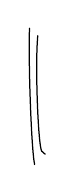
\begin{tikzpicture}[x=1cm,y=1cm,line width=.45pt,line cap=round]
\draw (0,0) .. controls (-.015,-.48) and (.025,-1.54) .. (.065,-1.73);
\draw (.105,-.095) .. controls (.070,-.48) and (.110,-1.48) .. (.155,-1.56) .. controls (.165,-1.58) and (.185,-1.59) .. (.200,-1.60);
\end{tikzpicture}}}}
\LMsourceMark{M000343}{\margin{\LMsourceMark{M000344}{\unsure{recall that we assume}} $\pi$ \LMsourceMark{M000345}{\unsure{anabelian|nonabelian}}
$(2g+\nu\geq3)$}}
\[
1\longrightarrow\pi'\longrightarrow
\widehat{\widehat{\mathcal T}}(\pi,i)\longrightarrow
\LMsourceMark{M000346}{\unsure{\widehat{\widehat{\mathcal G}}}}(\pi',i)\longrightarrow1
\]
or again
\[
1\longrightarrow\widehat{\pi}_{g,\nu-1}\longrightarrow
\widehat{\widehat{\mathcal T}}_{g,(\nu,\nu-1)}
\longrightarrow\LMsourceMark{M000347}{\unsure{\widehat{\widehat{\mathcal G}}}}_{g,\nu-1}
\longrightarrow1
\]
which contains the exact sequence
\[
1\longrightarrow\pi_{g,\nu-1}^{\LMsourceMark{M000348}{\unsure{*|+}}}\longrightarrow
\mathcal T_{g,(\nu,\nu-1)}\longrightarrow
\LMsourceMark{M000349}{\unsure{\mathcal G}}_{g,\nu-1}\longrightarrow1
\]
\LMsourceMark{M000350}{\unsure{as|known}} sub\var{\deleted{\LMsourceMark{M000351}{\unsure{particular|dense part}}}}{\LMsourceMark{M000352}{\LMcancelledDoubts{\LMsourceMark{M000353}{\unsure{particular|dense part}}}}}{deletion}{140-2-s348-D002}, \LMsourceMark{M000354}{\unsure{sequence|is}} exact.
It is convenient to work instead with
\diagram{\begin{tikzcd}[ampersand replacement=\&,column sep=2.1em,row sep=3.0em]
1 \arrow[r,dash] \&
\pi_{g,\nu-1} \arrow[r,dash] \arrow[d,hook',no head] \&
\LMsourceMark{M000355}{\unsure{\mathcal T}}_{g,\nu}^{!+} \arrow[r] \arrow[d,hook',no head] \&
\mathcal G_{g,\nu-1}^{!+} \arrow[r,dash] \arrow[d,hook',no head] \& 1 \\
1 \arrow[r,dash] \&
\widehat{\pi}_{g,\nu-1} \arrow[r] \arrow[d,equal] \&
\underset{\var{\deleted{\LMsourceMark{M000356}{\unsure{\LMsourceMark{M000357}{\illegible{1}}}}}}{\LMsourceMark{M000358}{\LMcancelledDoubts{\(\LMsourceMark{M000359}{\unsure{\LMsourceMark{M000360}{\illegible{1}}}}\)}}}{deletion}{140-2-s348-D003}}{\widehat{\mathcal T}_{g,\nu}^{!+}}
\arrow[r] \arrow[d,hook',no head] \&
\widehat{\mathcal G}_{g,\nu-1}^{!+} \arrow[r,dash] \arrow[d,hook'] \& 1 \\
1 \arrow[r,dash] \&
\widehat{\pi}_{g,\nu-1} \arrow[r] \&
\widehat{\widehat{\mathcal T}}_{g,\nu}^{!} \arrow[r] \&
\widehat{\widehat{\mathcal G}}_{g,\nu-1}^{!} \arrow[r,dash] \& 1
\end{tikzcd}}

The map \LMmathnotice{140-2-348-M1}
\begin{multline*}\LMsourceMark{M000361}{\unsure{\text{Prediscretifications}|\text{Prediscretifications}}}^{+}(\pi)\\\longrightarrow
\LMsourceMark{M000362}{\unsure{\text{Prediscretifications}|\text{Prediscretifications}}}^{+}(\pi')\end{multline*} is thus identified with
$\widehat{\widehat{\mathcal T}}_{g,\nu}^{!}/\widehat{\mathcal T}_{g,\nu}^{!}$,
we read off the diagram that this is
$\simeq\widehat{\widehat{\mathcal G}}_{g,\nu-1}^{\LMsourceMark{M000363}{\unsure{!}}\var{\deleted{\LMsourceMark{M000364}{\unsure{+}}}}{\LMsourceMark{M000365}{\LMcancelledDoubts{\(\LMsourceMark{M000366}{\unsure{+}}\)}}}{deletion}{140-2-s348-D004}}/
\widehat{\mathcal G}_{g,\nu-1}^{!+}$,
whence bijectivity on the sets of oriented prediscretifications.

In the group $\widehat{\widehat{\mathcal T}}_{g,\nu}^{!}=\mathcal T$,
we have an invariant subgroup $\widehat{\pi}_{g,\nu-1}=\pi'$,
and a subgroup $\Sigma$ $(\LMsourceMark{M000367}{\unsure{=|\longleftarrow}}\widehat{\mathcal T}_{g,\nu}^{!+})$
\LMsourceMark{M000368}{\mspage{347}}

\LMflushnotes\LMflushpages
\ifnum\LMform=1
\begin{LMapparatus}
\LMentry{140-2-s348-D001}{deletion}{\deleted{that}
}{\emph{\LMomittedlabel}}{Cancelled in the manuscript: omission follows the author's final state; uncertainty in the cancelled material remains marked.}{}
\LMentry{140-2-s348-D002}{deletion}{\deleted{\LMsourceMark{M000369}{\unsure{particular|dense part}}}
}{\emph{\LMomittedlabel}}{Cancelled in the manuscript: omission follows the author's final state; uncertainty in the cancelled material remains marked.}{}
\LMentry{140-2-s348-D003}{deletion}{\(\deleted{\LMsourceMark{M000370}{\unsure{\LMsourceMark{M000371}{\illegible{1}}}}}\)
}{\emph{\LMomittedlabel}}{Cancelled in the manuscript: omission follows the author's final state; uncertainty in the cancelled material remains marked.}{}
\LMentry{140-2-s348-D004}{deletion}{\(\deleted{\LMsourceMark{M000372}{\unsure{+}}}\)
}{\emph{\LMomittedlabel}}{Cancelled in the manuscript: omission follows the author's final state; uncertainty in the cancelled material remains marked.}{}
\end{LMapparatus}
\fi
\ifnum\LMform=2
\par\smallskip\begingroup\footnotesize\noindent\textcolor{gray}{\rule{.2\linewidth}{.35pt}}\par
\noindent\textit{\LMdoubtheading.}\par
\LMcarryover{140-2-s348-D002}{\LMsourceMark{M000373}{\unsure{particular|dense part}}
}
\LMcarryover{140-2-s348-D003}{\(\LMsourceMark{M000374}{\unsure{\LMsourceMark{M000375}{\illegible{1}}}}\)
}
\LMcarryover{140-2-s348-D004}{\(\LMsourceMark{M000376}{\unsure{+}}\)
}
\par\endgroup\smallskip
\fi

\ifnum\LMform=1
\par\begingroup\footnotesize
\noindent\texttt{140-2-348-M1} \textit{Layout placement}. The map with long alternative labels is displayed on two lines, broken before its arrow; marker M1 identifies the original running-text position.\par
\endgroup\fi
\LMsourceMark{M000377}{\scanpage{349}}

between $\pi'$ and $\mathcal T$, \var{\deleted{\LMsourceMark{M000378}{\unsure{giving by}}}}{\LMsourceMark{M000379}{\LMcancelledDoubts{\LMsourceMark{M000380}{\unsure{giving by}}}}}{deletion}{140-2-s349-D001} \var{\inserted{giving}}{\LMadded{giving}}{insertion}{140-2-s349-I001} a subgroup $\Sigma'\simeq\mathcal T(\pi')$\var{\inserted{$(=\LMsourceMark{M000381}{\unsure{\widehat{\mathcal G}^{!+}_{g,\nu-1}}})$}}{\LMadded{$(=\LMsourceMark{M000382}{\unsure{\widehat{\mathcal G}^{!+}_{g,\nu-1}}})$}}{insertion}{140-2-s349-I002} in $\LMsourceMark{M000383}{\unsure{\mathcal T'}}=\mathcal T/\pi'$ $(\simeq\widehat{\widehat{\mathcal G}}^{!}_{g,\nu-1})$, and we know well that then
\[
\mathcal T/\Sigma\simeq\mathcal T'/\Sigma',
\]
and \var{\deleted{$\LMsourceMark{M000384}{\unsure{N(\Sigma)}}$}}{\LMsourceMark{M000385}{\LMcancelledDoubts{\(\LMsourceMark{M000386}{\unsure{N(\Sigma)}}\)}}}{deletion}{140-2-s349-D002} that the normalizer \var{\inserted{$\mathcal N$,}}{\LMadded{$\mathcal N$,}}{insertion}{140-2-s349-I003} of $\Sigma$ in $\mathcal T$ is the inverse image of the normalizer $\mathcal N'$ of $\Sigma'$ in $\mathcal T'$, so that $\mathcal N/\Sigma\simeq\mathcal N'/\Sigma'$, which proves what we wanted.

\uline{Corollary} We have canonical \LMsourceMark{M000387}{\unsure{isomorphisms}}
\[
\Gamma_{g,\nu}\xrightarrow{\sim}\Gamma_{g,\nu-1}\xrightarrow{\sim}\LMsourceMark{M000388}{\unsure{\cdots}}\quad\var{\deleted{\LMsourceMark{M000389}{\unsure{\Gamma_{g,0}}}}}{\LMsourceMark{M000390}{\LMcancelledDoubts{\(\LMsourceMark{M000391}{\unsure{\Gamma_{g,0}}}\)}}}{deletion}{140-2-s349-D003}
\]
\LMsourceMark{M000392}{\margin{We also see that $\LMsourceMark{M000393}{\unsure{\Sigma|\Sigma^{!}}}$ invariant in $\LMsourceMark{M000394}{\unsure{\mathcal T|\widehat{\widehat{\mathcal T}}}}$ is equivalent to $\Sigma'$ invariant in $\widehat{\widehat{\mathcal T}}'$}}
so that if $g\geq2$, we have \LMsourceMark{M000395}{\unsure{canonically}} $\Gamma_{g,\nu}\simeq\Gamma_{g,0}$, on the other hand $\Gamma_{1,\nu}\simeq\Gamma_{1,1}$ $(g=1,\nu\geq1)$, $\Gamma_{0,\nu}\simeq\Gamma_{0,3}$ $(\nu\geq3)$.

\uline{N.B.} The ``fact'' \var{\deleted{\LMsourceMark{M000396}{\illegible{1}}}}{\LMsourceMark{M000397}{\LMcancelledDoubts{\LMsourceMark{M000398}{\illegible{1}}}}}{deletion}{140-2-s349-D004} assumed is far from obvious --- even that $\widehat{\widehat{\mathcal T}}^{\LMsourceMark{M000399}{\unsure{!}}}_{g,(\nu,\nu-1)}\longrightarrow\LMsourceMark{M000400}{\unsure{\widehat{\widehat{\mathcal T}}_{g,\nu-1}|\widehat{\widehat{\mathcal M}}_{g,\nu-1}}}$ is surjective, or that $\widehat{\widehat{\mathcal T}}_{g,(\nu,\nu-1)}\longrightarrow\widehat{\widehat{\mathcal G}}_{g,\nu-1}$ is injective, is far from obvious, and is perhaps altogether false !

The assumed fact amounts to a statement of the existence of a functor \LMsourceMark{M000401}{\unsure{in}} the opposite direction ``drilling holes'', \LMsourceMark{M000402}{\unsure{which|what}} in any case remains not understood.

\LMsourceMark{M000403}{\mspage{348}}

\LMflushnotes\LMflushpages
\ifnum\LMform=1
\begin{LMapparatus}
\LMentry{140-2-s349-D001}{deletion}{\deleted{\LMsourceMark{M000404}{\unsure{giving by}}}
}{\emph{\LMomittedlabel}}{Cancelled in the manuscript: omission follows the author's final state; uncertainty in the cancelled material remains marked.}{}
\LMentry{140-2-s349-I001}{insertion}{\inserted{giving}
}{\emph{\LMinsertedlabel}}{Explicit authorial insertion: integrated at the position recorded by the transcription, without changing its reading.}{}
\LMentry{140-2-s349-I002}{insertion}{\inserted{$(=\LMsourceMark{M000405}{\unsure{\widehat{\mathcal G}^{!+}_{g,\nu-1}}})$}
}{\emph{\LMinsertedlabel}}{Explicit authorial insertion: integrated at the position recorded by the transcription, without changing its reading.}{}
\LMentry{140-2-s349-D002}{deletion}{\deleted{$\LMsourceMark{M000406}{\unsure{N(\Sigma)}}$}
}{\emph{\LMomittedlabel}}{Cancelled in the manuscript: omission follows the author's final state; uncertainty in the cancelled material remains marked.}{}
\LMentry{140-2-s349-I003}{insertion}{\inserted{$\mathcal N$,}
}{\emph{\LMinsertedlabel}}{Explicit authorial insertion: integrated at the position recorded by the transcription, without changing its reading.}{}
\LMentry{140-2-s349-D003}{deletion}{\(\deleted{\LMsourceMark{M000407}{\unsure{\Gamma_{g,0}}}}\)
}{\emph{\LMomittedlabel}}{Cancelled in the manuscript: omission follows the author's final state; uncertainty in the cancelled material remains marked.}{}
\LMentry{140-2-s349-D004}{deletion}{\deleted{\LMsourceMark{M000408}{\illegible{1}}}
}{\emph{\LMomittedlabel}}{Cancelled in the manuscript: omission follows the author's final state; uncertainty in the cancelled material remains marked.}{}
\end{LMapparatus}
\fi
\ifnum\LMform=2
\par\smallskip\begingroup\footnotesize\noindent\textcolor{gray}{\rule{.2\linewidth}{.35pt}}\par
\noindent\textit{\LMdoubtheading.}\par
\LMcarryover{140-2-s349-D001}{\LMsourceMark{M000409}{\unsure{giving by}}
}
\LMcarryover{140-2-s349-D002}{\(\LMsourceMark{M000410}{\unsure{N(\Sigma)}}\)
}
\LMcarryover{140-2-s349-D003}{\(\LMsourceMark{M000411}{\unsure{\Gamma_{g,0}}}\)
}
\LMcarryover{140-2-s349-D004}{\LMsourceMark{M000412}{\illegible{1}}
}
\par\endgroup\smallskip
\fi

\LMsourceMark{M000413}{\scanpage{350}}
\LMsourceMark{M000414}{\mspage{177}}

28. \uline{Change of type} $(g,\nu)$ \LMsourceMark{M000415}{\unsure{(continued)}} : \uline{\LMsourceMark{M000416}{\unsure{passage}} to a finite covering.}

Let $\pi$ be a profinite group \var{\inserted{with loops}}{\LMadded{with loops}}{insertion}{140-2-s350-I001} of type $(g,\nu)$, anabelian as always, $\pi'$ a subgroup of finite index. We know (\LMsourceMark{M000417}{\unsure{or we|we thereby}} verify, by passing to the discrete case) that \var{\deleted{\LMsourceMark{M000418}{\illegible{1}} \LMsourceMark{M000419}{\unsure{discretified}}}}{\LMsourceMark{M000420}{\LMcancelledDoubts{\LMsourceMark{M000421}{\illegible{1}}\quad \LMsourceMark{M000422}{\unsure{discretified}}}}}{deletion}{140-2-s350-D001} \var{\inserted{equipped with the}}{\LMadded{equipped with the}}{insertion}{140-2-s350-I002} \LMsourceMark{M000423}{\unsure{traces}} \LMsourceMark{M000424}{\unsure{on|under}} $\pi$ of the \LMsourceMark{M000425}{\unsure{loop}} subgroups of $\pi$, $\pi'$ is a group with loops.

\var{\deleted{If for every $i\in I(\pi)$, we consider an $L_i$, and the $\LMsourceMark{M000426}{\unsure{n}}$ conjugates $\LMsourceMark{M000427}{\unsure{\operatorname{int}(g)}}L_i$ \inserted{$=L_{i\alpha}$}, with $g\in\pi\bmod\pi'$ $(n=[\pi:\pi']\LMsourceMark{M000428}{\unsure{\}}},\ \deleted{\LMsourceMark{M000429}{\unsure{n}}}\ \inserted{1\leq\alpha\leq n})$ \deleted{\LMsourceMark{M000430}{\unsure{counted|to count}} the number of times that a conjugacy class in $\pi'$ of the subgroup $\LMsourceMark{M000431}{\unsure{\operatorname{int}(g)}}L_i$ is} \inserted{then if $\LMsourceMark{M000432}{\unsure{d_{\alpha}|d_{i\alpha}}}=[L_{i\alpha}:\LMsourceMark{M000433}{\unsure{L'_{i\alpha}|N'_{i\alpha}}}\deleted{\LMsourceMark{M000434}{\unsure{\cap\pi'}}}]$ \LMsourceMark{M000435}{\unsure{for}} $L'_{i\alpha}=L_{i\alpha}\cap\pi'$, then} exactly $d_{i\alpha}$ among the $L'_{i\beta}$ \inserted{$(1\leq\beta\leq n)$} are conjugate in $\pi'$ to $L'_{i\alpha}$, and if we sum over the distinct \LMsourceMark{M000436}{\unsure{conjugacy}} classes of the subgroups}}{\LMsourceMark{M000437}{\LMcancelledDoubts{\(\LMsourceMark{M000438}{\unsure{n}}\)\quad \(\LMsourceMark{M000439}{\unsure{\operatorname{int}(g)}}\)\quad \(\LMsourceMark{M000440}{\unsure{\}}}\)\quad \(\LMsourceMark{M000441}{\unsure{n}}\)\quad \LMsourceMark{M000442}{\unsure{counted|to count}}\quad \(\LMsourceMark{M000443}{\unsure{\operatorname{int}(g)}}\)\quad \(\LMsourceMark{M000444}{\unsure{d_{\alpha}|d_{i\alpha}}}\)\quad \(\LMsourceMark{M000445}{\unsure{L'_{i\alpha}|N'_{i\alpha}}}\)\quad \(\LMsourceMark{M000446}{\unsure{\cap\pi'}}\)\quad \LMsourceMark{M000447}{\unsure{for}}\quad \LMsourceMark{M000448}{\unsure{conjugacy}}}}}{deletion}{140-2-s350-D002}

The loop subgroups are \LMsourceMark{M000449}{\unsure{also|thus}} the \var{\deleted{\LMsourceMark{M000450}{\unsure{the}}}}{\LMsourceMark{M000451}{\LMcancelledDoubts{\LMsourceMark{M000452}{\unsure{the}}}}}{deletion}{140-2-s350-D006} subgroups $L'$ such that
\[
\text{a)}\quad L'=\operatorname{Centr}_{\pi}(L')\cap\pi'.
\]
\[
\text{b)}\quad L\LMsourceMark{M000453}{\unsure{=|:}}\operatorname{Centr}_{\pi}(L')\text{ is a \LMsourceMark{M000454}{\unsure{loop}} subgroup in }\pi.
\]
We put $d(L')=[L:L']$, and we thus have a function
\[
d:I'=I(\pi')\longrightarrow\mathbb N^*,
\]
and a map $I'\xrightarrow{\varphi}I$, such that $\forall i\in I$, we have
\[
\text{(1)}\qquad \sum_{\substack{i'\in I'\\\text{over }i}}d(i')=n
\qquad (\text{\LMsourceMark{M000455}{\unsure{where|here}}}\ n=[\pi:\pi'])
\]
We will have the Hurwitz formula
\[
\text{(2)}\qquad \var{\deleted{\LMsourceMark{M000456}{\unsure{2g|2\alpha}}}}{\LMsourceMark{M000457}{\LMcancelledDoubts{\(\LMsourceMark{M000458}{\unsure{2g|2\alpha}}\)}}}{deletion}{140-2-s350-D007}\ 2g'-2=n(2g-2)+\overbrace{\sum_{i'\in I'}(d(i')-1)}^{\var{\inserted{n\operatorname{card}I-\operatorname{card}I'}}{\LMadded{n\operatorname{card}I-\operatorname{card}I'}}{insertion}{140-2-s350-I007}}
\]
\LMsourceMark{M000459}{\mspage{349}}

\LMflushnotes\LMflushpages
\ifnum\LMform=1
\begin{LMapparatus}
\LMentry{140-2-s350-I001}{insertion}{\inserted{with loops}
}{\emph{\LMinsertedlabel}}{Explicit authorial insertion: integrated at the position recorded by the transcription, without changing its reading.}{}
\LMentry{140-2-s350-D001}{deletion}{\deleted{\LMsourceMark{M000460}{\illegible{1}} \LMsourceMark{M000461}{\unsure{discretified}}}
}{\emph{\LMomittedlabel}}{Cancelled in the manuscript: omission follows the author's final state; uncertainty in the cancelled material remains marked.}{}
\LMentry{140-2-s350-I002}{insertion}{\inserted{equipped with the}
}{\emph{\LMinsertedlabel}}{Explicit authorial insertion: integrated at the position recorded by the transcription, without changing its reading.}{}
\LMentry{140-2-s350-D002}{deletion}{\deleted{If for every $i\in I(\pi)$, we consider an $L_i$, and the $\LMsourceMark{M000462}{\unsure{n}}$ conjugates $\LMsourceMark{M000463}{\unsure{\operatorname{int}(g)}}L_i$ \inserted{$=L_{i\alpha}$}, with $g\in\pi\bmod\pi'$ $(n=[\pi:\pi']\LMsourceMark{M000464}{\unsure{\}}},\ \deleted{\LMsourceMark{M000465}{\unsure{n}}}\ \inserted{1\leq\alpha\leq n})$ \deleted{\LMsourceMark{M000466}{\unsure{counted|to count}} the number of times that a conjugacy class in $\pi'$ of the subgroup $\LMsourceMark{M000467}{\unsure{\operatorname{int}(g)}}L_i$ is} \inserted{then if $\LMsourceMark{M000468}{\unsure{d_{\alpha}|d_{i\alpha}}}=[L_{i\alpha}:\LMsourceMark{M000469}{\unsure{L'_{i\alpha}|N'_{i\alpha}}}\deleted{\LMsourceMark{M000470}{\unsure{\cap\pi'}}}]$ \LMsourceMark{M000471}{\unsure{for}} $L'_{i\alpha}=L_{i\alpha}\cap\pi'$, then} exactly $d_{i\alpha}$ among the $L'_{i\beta}$ \inserted{$(1\leq\beta\leq n)$} are conjugate in $\pi'$ to $L'_{i\alpha}$, and if we sum over the distinct \LMsourceMark{M000472}{\unsure{conjugacy}} classes of the subgroups}
}{\emph{\LMomittedlabel}}{Cancelled in the manuscript: omission follows the author's final state; uncertainty in the cancelled material remains marked.}{}
\LMentry{140-2-s350-D006}{deletion}{\deleted{\LMsourceMark{M000473}{\unsure{the}}}
}{\emph{\LMomittedlabel}}{Cancelled in the manuscript: omission follows the author's final state; uncertainty in the cancelled material remains marked.}{}
\LMentry{140-2-s350-D007}{deletion}{\(\deleted{\LMsourceMark{M000474}{\unsure{2g|2\alpha}}}\)
}{\emph{\LMomittedlabel}}{Cancelled in the manuscript: omission follows the author's final state; uncertainty in the cancelled material remains marked.}{}
\LMentry{140-2-s350-I007}{insertion}{\(\inserted{n\operatorname{card}I-\operatorname{card}I'}\)
}{\emph{\LMinsertedlabel}}{Explicit authorial insertion: integrated at the position recorded by the transcription, without changing its reading.}{}
\end{LMapparatus}
\fi
\ifnum\LMform=2
\par\smallskip\begingroup\footnotesize\noindent\textcolor{gray}{\rule{.2\linewidth}{.35pt}}\par
\noindent\textit{\LMdoubtheading.}\par
\LMcarryover{140-2-s350-D001}{\LMsourceMark{M000475}{\illegible{1}}\quad \LMsourceMark{M000476}{\unsure{discretified}}
}
\LMcarryover{140-2-s350-D002}{\(\LMsourceMark{M000477}{\unsure{n}}\)\quad \(\LMsourceMark{M000478}{\unsure{\operatorname{int}(g)}}\)\quad \(\LMsourceMark{M000479}{\unsure{\}}}\)\quad \(\LMsourceMark{M000480}{\unsure{n}}\)\quad \LMsourceMark{M000481}{\unsure{counted|to count}}\quad \(\LMsourceMark{M000482}{\unsure{\operatorname{int}(g)}}\)\quad \(\LMsourceMark{M000483}{\unsure{d_{\alpha}|d_{i\alpha}}}\)\quad \(\LMsourceMark{M000484}{\unsure{L'_{i\alpha}|N'_{i\alpha}}}\)\quad \(\LMsourceMark{M000485}{\unsure{\cap\pi'}}\)\quad \LMsourceMark{M000486}{\unsure{for}}\quad \LMsourceMark{M000487}{\unsure{conjugacy}}
}
\LMcarryover{140-2-s350-D006}{\LMsourceMark{M000488}{\unsure{the}}
}
\LMcarryover{140-2-s350-D007}{\(\LMsourceMark{M000489}{\unsure{2g|2\alpha}}\)
}
\par\endgroup\smallskip
\fi

% END PACKAGE LM_P035
\end{document}
